\documentclass[11pt]{article}
\usepackage[utf8]{inputenc}
\usepackage[T2A]{fontenc}
\usepackage[russian]{babel}
\usepackage{amsmath,amssymb,amsthm}
\usepackage[a4paper,left=24mm,right=20mm,top=22mm,bottom=24mm]{geometry}
\usepackage{graphicx}
\usepackage{array}
\usepackage{booktabs}
\usepackage{enumitem}
\usepackage[dvipsnames,table]{xcolor}
\usepackage{mdframed}
\usepackage[colorlinks=true,linkcolor=NavyBlue,citecolor=BrickRed,urlcolor=NavyBlue]{hyperref}

\newtheorem{theorem}{Теорема}
\newtheorem{lemma}{Лемма}
\newtheorem{proposition}{Предложение}
\newtheorem{corollary}{Следствие}
\theoremstyle{definition}
\newtheorem{definition}{Определение}
\theoremstyle{remark}
\newtheorem{remark}{Замечание}

\newcommand{\R}{\mathbb{R}}
\newcommand{\Z}{\mathbb{Z}}
\newcommand{\E}{\mathbb{E}}
\newcommand{\diam}{\operatorname{diam}}
\newcommand{\dist}{\operatorname{dist}}
\newcommand{\vol}{\operatorname{vol}}

% рамка для ключевых утверждений
\newmdenv[linecolor=NavyBlue!60,linewidth=0.8pt,backgroundcolor=NavyBlue!4,
  roundcorner=4pt,skipabove=8pt,skipbelow=8pt,innertopmargin=6pt,
  innerbottommargin=6pt]{keybox}

\title{\bfseries Верхние оценки $\chi(\R^4)\le 45$, $\chi(\R^5)\le132$\\
и $\chi(\R^7)\le 1323$\\[2pt]
\large решётки общего положения и точные ширины запрещённых интервалов%
\thanks{Черновик от 05.08.2026. Аффилиации и контактные данные авторов подлежат
уточнению. Все вычислительные скрипты, точные сертификаты и промежуточные данные
приложены к репозиторию проекта (пакеты \texttt{voronoi4d} и \texttt{combigeo},
каталог \texttt{audit-data}); репозиторий открывается одновременно с публикацией.}}
\author{Л.\,Л.~Иванов \and Н.~Глушкова}
\date{5 августа 2026 г.}

\begin{document}
\maketitle


\begin{abstract}
\noindent
Раскраска евклидова пространства называется \emph{правильной для запрещённого
отрезка расстояний} $[1,\ell]$, если никакие две одноцветные точки не находятся
на расстоянии из $[1,\ell]$; наименьшее необходимое число цветов обозначается
$\chi\bigl(\R^n,[1,\ell]\bigr)$, а при $\ell=1$ --- это классическое
хроматическое число $\chi(\R^n)$ (проблема Нельсона--Хадвигера).

Мы строим три новые решёточные раскраски: в \textbf{45} цветов для $\R^4$
(правильную при $\ell\le1{,}015$), в \textbf{132} цвета для $\R^5$
($\ell\le1{,}01$) и в \textbf{1323} цвета для $\R^7$ ($\ell\le1{,}007$). В
частности, $\chi(\R^4)\le45$, $\chi(\R^5)\le132$ и $\chi(\R^7)\le1323$, что
улучшает известные оценки $49$, $140$ и $1372$. Тем самым опровергается
ожидание Армана, Бондаренко, Прымака и Радченко, что $49$ и $140$ --- минимумы
среди всех решёточных раскрасок $\R^4$ и $\R^5$.

Все три раскраски задаются решётками \emph{общего положения}, найденными
оптимизацией самой метрики; именно выход за пределы классических решёток
($D_4$, $A_4^*$, $A_5^*$, $E_7^*$) делает улучшение возможным. Ключевые
неравенства доказаны в \emph{точной рациональной арифметике}, поэтому
результаты не зависят от вычислений с плавающей точкой.

Дополнительно приведена раскраска, дающая $\chi\bigl(\R^4,[1,\ell]\bigr)\le48$
для более широкого интервала $\ell\le1{,}0396$, вычислены точные ширины
запрещённых интервалов всех конструкций Армана и др. в размерностях
$4\le n\le9$, для эйзенштейновых конструкций получено тождество, реализующее
усиление из замечания~9 той же работы, и уточнены наши прежние табличные
результаты для $\R^3$.
\end{abstract}


\tableofcontents
\medskip


\section{Введение}\label{sec:intro}

\subsection{Задача}

\emph{Хроматическим числом плоскости} $\chi(\R^2)$ называется наименьшее число
цветов, в которые можно окрасить все точки плоскости так, чтобы никакие две
точки на расстоянии ровно~$1$ не оказались одного цвета. Этот вопрос, известный
как \emph{проблема Нельсона--Хадвигера} (ок.~$1950$), до сих пор не решён: с
$2018$~г. известно лишь $5\le\chi(\R^2)\le7$ \cite{deGrey,Soifer}. Аналогично
определяется $\chi(\R^n)$ для пространства любой размерности.

Естественное обобщение --- запрещать не одно расстояние, а целый \emph{отрезок}:
через $\chi\bigl(\R^n,[1,\ell]\bigr)$ обозначим наименьшее число цветов
раскраски, при которой одноцветные точки не реализуют ни одного расстояния из
отрезка $[1,\ell]$, $\ell\ge1$. При $\ell=1$ отрезок вырождается в точку и мы
возвращаемся к классическому $\chi(\R^n)=\chi\bigl(\R^n,[1,1]\bigr)$.
Систематическое изучение версии с интервалом начато одним из авторов
в~\cite{Ivanov2011}. Поскольку запрет более широкого множества расстояний требует
не меньше цветов,
\begin{equation}\label{eq:mono}
\chi(\R^n)=\chi\bigl(\R^n,[1,1]\bigr)\ \le\ \chi\bigl(\R^n,[1,\ell]\bigr)
\qquad(\ell\ge1),
\end{equation}
и любая оценка сверху для интервальной версии автоматически оценивает
классическое хроматическое число.

\subsection{Известные оценки}

Все известные \emph{верхние} оценки $\chi(\R^n)$ в малых размерностях получены
по существу одним геометрическим приёмом --- \emph{периодической раскраской по
разбиению Вороного некоторой решётки} (см.~\S\ref{sec:method}). Приведём
современное состояние (нижние границы --- для контекста):
\[
\begin{array}{r|l|l}
n & \text{нижняя граница} & \text{верхняя граница}\\\hline
2 & 5\ \text{\cite{deGrey}} & 7\ \text{(Исбелл; см.~\cite{Soifer})}\\
3 & 6\ \text{\cite{Nechushtan}} & 15\ \text{\cite{Coulson}}\\
4 & 9\ \text{\cite{ExooIsmailescu}} & \mathbf{45}\ \text{(наст. работа; было }49\text{)}\\
5 & 9\ \text{\cite{Cantwell}} & \mathbf{132}\ \text{(наст. работа; было }140\text{)}\\
6 & 12\ \text{\cite{ExooIsmailescu2014}} & 343\ \text{\cite{ABPR}}\\
7 & 16\ \text{\cite{ExooIsmailescu2014}} & \mathbf{1323}\ \text{(наст. работа; было }1372\text{)}
\end{array}
\]
Верхняя оценка в размерности~4 имеет историю: $\le54$ (Радоичич, Тот
\cite{RadoicicToth}, решётка $A_4^*$); оценка $\le49$ заявлена без доказательства
Кулсоном и приведена в \cite{CoulsonPayne2007}; полное доказательство, вместе с
проверкой минимальности индекса~$49$ \emph{для решётки $D_4$}, дано Арманом,
Бондаренко, Прымаком и Радченко \cite{ABPR} (далее --- АБПР). Нижняя граница в
этой размерности прошла путь $6$ (Райский) $\to7$ \cite{Ivanov2006}
$\to9$ \cite{ExooIsmailescu}. В той же работе (открытый вопрос~1) высказано ожидание, что улучшить $49$
нельзя:
\begin{quote}\itshape\small
<<We believe that the answer is negative for $n=4,5$, i.e.
$\min\chi_s(\E^4,\Lambda,\Lambda',\ell)=49$~\ldots>> (\cite{ABPR}, Open
question~1),
\end{quote}
где минимум берётся по всем решёткам $\Lambda$, подрешёткам $\Lambda'$ и всем
$\ell>0$. Настоящая работа опровергает это ожидание.

\subsection{Результаты}

\begin{keybox}
\textbf{Основные результаты.} $\chi(\R^4)\le 45$; точнее,
$\chi\bigl(\R^4,[1,\ell]\bigr)\le45$ при всех $\ell\le1{,}015$
(теорема~\ref{thm:main}). Раскраска решёточная, задаётся явной рациональной
решёткой общего положения; ключевое неравенство доказано в точной рациональной
арифметике (\S\ref{sec:comp}). Кроме того,
$\chi\bigl(\R^5,[1,\ell]\bigr)\le132$ при $\ell\le1{,}01$, в частности
$\chi(\R^5)\le132$ (теорема~\ref{thm:r5}), и
$\chi\bigl(\R^7,[1,\ell]\bigr)\le1323$ при $\ell\le1{,}007$, в частности
$\chi(\R^7)\le1323$ (теорема~\ref{thm:r7}); обе новые конструкции имеют
рациональные компьютерно проверяемые сертификаты.
\end{keybox}

\noindent Кроме того:
\begin{itemize}[leftmargin=1.4em,itemsep=1pt]
\item раскраска в $48$ цветов, правильная для более широкого интервала
$\ell\le1{,}0396$ (\S\ref{sec:wide}), --- компромисс <<меньше цветов ${}\leftrightarrow{}$
шире интервал>>, ранее не отмечавшийся;
\item точные ширины запрещённых интервалов \emph{всех} явных конструкций АБПР в
размерностях $4\le n\le9$ (\S\ref{sec:extra}; в \cite{ABPR} доказывалось лишь
$\ge1$), и тождество $D=\sqrt{7/3}\,\lambda_1$ для эйзенштейновых конструкций,
дающее их точную ширину и явно реализующее усиление из замечания~9
работы~\cite{ABPR};
\item уточнение (в большую сторону) нашей прежней таблицы \cite{Ivanov2011}
для $\R^3$ и исправление трёх допущенных в ней опечаток;
\item масштабируемый метод поиска раскрасок для $n\ge5$: точное исправление
детерминанта по кофактору, CSP и min-conflicts, доводка по активному набору с доверительной областью, температурное продолжение метрики и безвершинное вычисление радиуса покрытия
(\S\ref{sec:big});
\item полный поиск по примарным CRT-блокам, пороговое расширение портфеля
дискретных бассейнов и дискретно-непрерывное чередование ядра и формы Грама,
понижающие оценку для $\R^5$ с $140$ до $132$ и опровергающие прежнюю
диагностику <<неустранимого>> единичного конфликта;
\item примарный Radon/FFT-поиск по полным блокам характеров конечных полей и
геометрически взвешенная целевая функция, которые совместно с деформацией формы
Грама понижают оценку в $\R^7$ с $1372$ до $1323$; прежние отрицательные
эксперименты на фиксированной $E_7^*$ объясняют, почему необходимы обе стадии
(\S\ref{sec:big});
\item лестницы ширин в $\R^5$ и $\R^6$ (табл.~\ref{tab:stair56}) и
воспроизводимые отрицательные экраны ближайших индексов в размерностях
$6$--$9$, не трактуемые как доказательства невозможности;
\item свободно доступная реализация всего конвейера (\S\ref{sec:algo}) с
многопоточным перебором и точной сертификацией.
\end{itemize}

\medskip\noindent
\textbf{Шкала статусов.} Работа сочетает доказательства, точные компьютерные
сертификаты и обширный численный поиск, поэтому всюду ниже утверждения
помечены одной из четырёх меток:

\begin{description}[leftmargin=2.4em,itemsep=1pt,topsep=3pt]
\item[\textbf{[Т]}] \emph{теорема} --- доказано обычными средствами;
\item[\textbf{[С]}] \emph{точный сертификат} --- сведено к конечному набору
неравенств между рациональными числами, проверенных в точной арифметике дробей;
плавающая точка могла участвовать в \emph{выборе} кандидатов, но не в проверке;
\item[\textbf{[Ч]}] \emph{численный результат} --- получено вычислениями с
плавающей точкой; приводится как ориентир, доказательной силы не имеет;
\item[\textbf{[Э]}] \emph{экран} --- перебор, завершившийся \emph{отрицательно}
и \emph{на фиксированной численной форме}. Экран не является доказательством
невозможности: изменение формы Грама выводит из перебранного множества.
\end{description}

\noindent Все три оценки заголовка имеют статус \textbf{[С]}.


\section{Метод: раскраска по решёткам Вороного}\label{sec:method}

\subsection{Решётки, подрешётки, ячейки Вороного}

\emph{Решётка} $\Lambda\subset\R^n$ --- это множество всех целочисленных
линейных комбинаций $n$ линейно независимых векторов $b_1,\dots,b_n$ (базиса);
геометрически это регулярная <<кристаллическая>> сетка узлов. \emph{Подрешётка}
$\Gamma\subseteq\Lambda$ --- решётка, все узлы которой лежат в $\Lambda$; её
\emph{индекс} $k=[\Lambda:\Gamma]$ равен числу классов смежности
$\Lambda/\Gamma$ (во сколько раз $\Gamma$ <<реже>> $\Lambda$) и вычисляется как
модуль определителя целочисленной матрицы перехода.

\emph{Ячейкой Вороного} узла $a\in\Lambda$ называется множество точек
пространства, для которых $a$ --- ближайший узел решётки:
\[
V_\Lambda(a)=\{x\in\R^n:\ \|x-a\|\le\|x-b\|\ \ \forall b\in\Lambda\}.
\]
Это выпуклый многогранник (для плоской шестиугольной решётки ---
правильный шестиугольник, рис.~\ref{fig:method}); все ячейки одинаковы с
точностью до сдвига и вместе замощают $\R^n$ без пробелов. Обозначим
$V_0=V_\Lambda(0)$ --- центральную ячейку.

\begin{figure}[t]
\centering
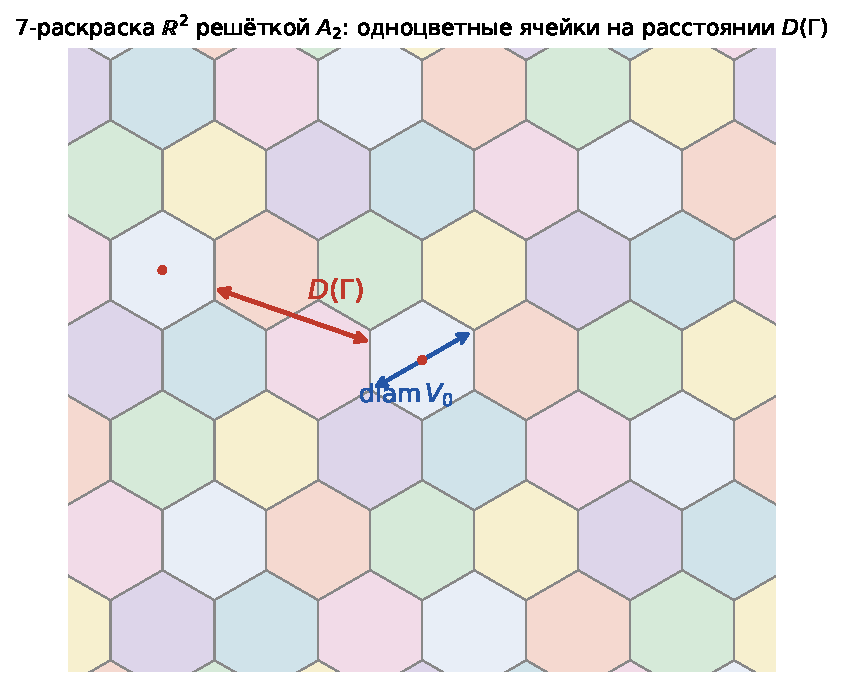
\includegraphics[width=0.66\textwidth]{fig_method.pdf}
\caption{Идея метода на примере $7$-раскраски плоскости шестиугольной решёткой
$A_2$ (классическая конструкция Исбелла, дающая $\chi(\R^2)\le7$). Каждая ячейка
Вороного (шестиугольник) окрашена цветом своего класса смежности по подрешётке
индекса~$7$; всего $7$ цветов. Две \emph{одноцветные} ячейки (красные точки)
разделены расстоянием $D(\Gamma)$, строго большим диаметра ячейки
$\diam V_0$. Раскраска запрещает все расстояния из промежутка
$\bigl(\diam V_0,\,D(\Gamma)\bigr)$.}
\label{fig:method}
\end{figure}

\subsection{Раскраска классами смежности}

Зафиксируем подрешётку $\Gamma\subseteq\Lambda$ индекса $k$ и окрасим каждую
ячейку $V_\Lambda(v)$ цветом класса смежности $v+\Gamma$. Так как классов ровно
$k$, получается $k$-цветная периодическая раскраска всего $\R^n$
(рис.~\ref{fig:method}). Ключевой вопрос: \emph{какие расстояния могут
разделять две одноцветные точки?}

Две точки одного цвета лежат либо в одной ячейке, либо в ячейках
$V_\Lambda(a)$, $V_\Lambda(b)$, центры которых отличаются на ненулевой вектор
$v=a-b\in\Gamma$. В первом случае расстояние не превосходит диаметра
$\diam V_0$; во втором --- не меньше расстояния между этими двумя ячейками.
Обозначим
\[
D(v)=\dist\bigl(V_0,\,v+V_0\bigr),\qquad
D(\Gamma)=\min_{v\in\Gamma\setminus\{0\}}D(v).
\]
Тогда множество \emph{реализуемых} одноцветных расстояний целиком лежит в
\[
[0,\ \diam V_0]\ \cup\ [D(\Gamma),\ \infty),
\]
а открытый промежуток $\bigl(\diam V_0,\,D(\Gamma)\bigr)$ \emph{свободен} ---
ни одна пара одноцветных точек не находится на таком расстоянии
(рис.~\ref{fig:interval}). Масштабируя решётку, этот свободный промежуток можно
совместить с любым наперёд заданным отрезком $[1,\ell]$, лишь бы отношение
\begin{equation}\label{eq:d-def}
d(\Lambda,\Gamma)\ :=\ \frac{D(\Gamma)}{\diam V_0}
\end{equation}
превосходило~$1$.

\begin{figure}[t]
\centering
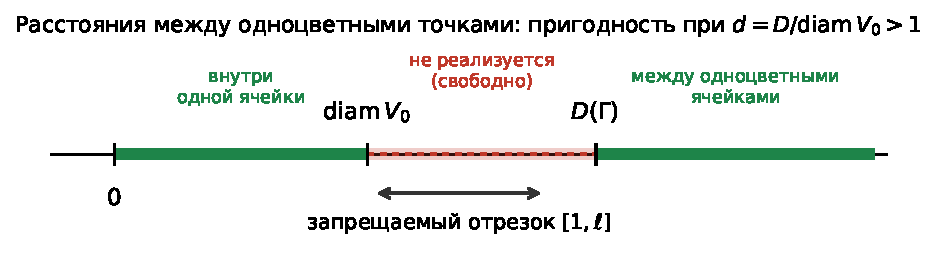
\includegraphics[width=0.86\textwidth]{fig_interval.pdf}
\caption{Расстояния между одноцветными точками (числовая ось). Реализуются лишь
малые (внутри одной ячейки, $\le\diam V_0$) и большие (между разными
одноцветными ячейками, $\ge D(\Gamma)$); промежуток между ними свободен. Если
$d=D(\Gamma)/\diam V_0>1$, то после нормировки $\diam V_0\mapsto{}$<<чуть меньше
$1$>> весь отрезок $[1,\ell]$ с $\ell<d$ попадает в свободную зону --- раскраска
правильна для $[1,\ell]$.}
\label{fig:interval}
\end{figure}

\begin{proposition}\label{prop:crit}
Если $d(\Lambda,\Gamma)>1$, то $\chi\bigl(\R^n,[1,\ell]\bigr)\le[\Lambda:\Gamma]$
при всех $\ell<d(\Lambda,\Gamma)$; в частности $\chi(\R^n)\le[\Lambda:\Gamma]$.
\end{proposition}
\begin{proof}
Возьмём масштаб $s>0$ с $s\,\diam V_0<1$ и $s\,D(\Gamma)>\ell$ --- это возможно
тогда и только тогда, когда $\ell<D(\Gamma)/\diam V_0=d$. Для решётки $s\Lambda$
свободный промежуток $\bigl(s\diam V_0,\,sD(\Gamma)\bigr)$ содержит весь отрезок
$[1,\ell]$, значит раскраска правильна для $[1,\ell]$. Случай $\ell=1$ (с учётом
\eqref{eq:mono}) даёт $\chi(\R^n)\le k$.
\end{proof}

Таким образом, вся задача сводится к поиску пары <<решётка + подрешётка>> с
возможно большим отношением~\eqref{eq:d-def}. Величину $d$ будем называть
\emph{нормированной шириной} (запрещённого интервала); чем она больше при данном
числе цветов $k$, тем сильнее оценка.

\subsection{Как считать $D(v)$: лемма о середине}

Прямое вычисление расстояния между двумя многогранниками --- задача негладкой
оптимизации. В~\cite{Ivanov2011} она сведена к расстоянию \emph{от точки до
одного многогранника} с помощью центральной симметрии ячеек Вороного
(классическое свойство, восходящее к Вороному \cite{Voronoi}).

\begin{lemma}[Вороной]\label{lem:sym}
Ячейка $V_0$ --- выпуклый центрально-симметричный многогранник, и все её грани
центрально-симметричны.
\end{lemma}

\begin{lemma}[о середине; {\cite[лемма~2]{Ivanov2011}}]\label{lem:mid}
Минимальное расстояние между ячейками $V_0$ и $v+V_0$ реализуется на паре
точек, симметричных относительно середины $v/2$ отрезка их центров. Как
следствие,
\begin{equation}\label{eq:mid}
D(v)=2\,\dist\bigl(v/2,\,V_0\bigr).
\end{equation}
\end{lemma}
\begin{proof}[Идея]
Пусть минимум достигается на $x\in V_0$, $y\in v+V_0$. Отражение через $v/2$
переводит (в силу леммы~\ref{lem:sym}) $V_0$ в $v+V_0$ и наоборот; образы
$x',y'$ дают ту же длину $|x'-y'|=|x-y|$. Середины отрезков $[x,y']$ и $[y,x']$
по выпуклости лежат в соответствующих ячейках, симметричны относительно $v/2$ и
реализуют то же минимальное расстояние. Значит, минимум достигается на
симметричной паре, а расстояние от каждой точки до $v/2$ равно $\dist(v/2,V_0)$.
\end{proof}

Формула~\eqref{eq:mid} превращает вычисление $D(v)$ в стандартную задачу
<<расстояние от точки до выпуклого многогранника>>.

\subsection{Полнота перебора соседей}

Минимум $D(\Gamma)=\min_v D(v)$ берётся по бесконечной подрешётке, но
перебирать нужно лишь \emph{конечное} множество коротких векторов. Так как
$V_0$ содержится в шаре радиуса $\tfrac12\diam V_0$, справедлива нижняя оценка
$D(v)\ge\|v\|-\diam V_0$. Поэтому если уже найден некоторый вектор с $D=D_{*}$,
то улучшить минимум могут только векторы с
\begin{equation}\label{eq:window}
\|v\|\ <\ D_{*}+\diam V_0.
\end{equation}
Это \emph{доказуемо полная} граница перебора (в отличие от эвристических
<<окон>>): она справедлива при любом базисе подрешётки и гарантирует, что ни
один потенциально лучший сосед не пропущен.

Наименьшее число цветов среди раскрасок описанного вида --- то есть минимум
$[\Lambda:\Gamma]$ по всем решёткам $\Lambda$, подрешёткам $\Gamma$ и
масштабам --- принято обозначать $\chi_s\bigl(\R^n,[1,\ell]\bigr)$; очевидно,
$\chi\bigl(\R^n,[1,\ell]\bigr)\le\chi_s\bigl(\R^n,[1,\ell]\bigr)$. Все
известные верхние оценки в малых размерностях, включая полученные ниже, --- это
оценки на $\chi_s$.

\begin{remark}[о границах ячеек]\label{rem:halfopen}
Ячейки Вороного замкнуты и пересекаются по границам, поэтому <<окрасим каждую
ячейку>> само по себе не задаёт функцию на $\R^n$. Как обычно, мы фиксируем
полуоткрытую фундаментальную область: из каждой пары соседних ячеек общая грань
приписывается одной из них. Все оценки ниже от этого выбора не зависят, так как
диаметр полуоткрытой ячейки не превосходит $\diam V_0$, а расстояние между
разноимёнными ячейками не меньше $D(v)$.
\end{remark}


\section{Алгоритм и его реализация}\label{sec:algo}

Опишем концептуально вычислительный конвейер; технические детали и код --- в
пакетах \texttt{voronoi4d} (эталонная реализация на Python) и \texttt{combigeo}
(быстрое ядро на C++), включённых в репозиторий проекта.

\paragraph{(1) Приведение базиса.} Базис решётки предварительно
\emph{LLL-приводится} --- заменяется на эквивалентный, но <<почти
ортогональный>>, с короткими векторами (алгоритм Ленстры--Ленстры--Ловаса
\cite{LLL}). Это резко сужает все последующие переборы.

\paragraph{(2) Построение ячейки Вороного.} Грани ячейки задаются
\emph{релевантными векторами} решётки. По теореме Вороного релевантные векторы
--- это кратчайшие представители ненулевых классов смежности $\Lambda/2\Lambda$
(их не более $2(2^n-1)$); мы находим их точным перебором ближайших векторов
(\emph{CVP}, задача о ближайшем векторе, методом сферического декодирования
Финке--Поста \cite{FinckePohst}) в каждом из $2^n-1$ классов. По найденным
граням перечисляются вершины ячейки. Корректность построенной ячейки
контролируется независимо: проверяется соотношение Эйлера для её $f$-вектора,
центральная симметрия множества вершин и равенство её объёма определителю
решётки. Полнота самого списка вершин контролируется тождеством
\begin{equation}\label{eq:vertsum}
\sum_{x\in\mathrm{vert}\,V_0}\bigl|\det(v_1,\dots,v_n)\bigr|=(n+1)!,
\end{equation}
где $v_1,\dots,v_n$ --- релевантные векторы фасет, активных в вершине~$x$: слева
стоит сумма нормированных объёмов симплексов Делоне, инцидентных узлу решётки, а
она не зависит от комбинаторного типа ячейки. Для примитивной решётки все
слагаемые равны~$1$ и вершин ровно $(n+1)!$; в общем случае вершин меньше, и
\eqref{eq:vertsum} даёт проверяемое равенство вместо ссылки на связность графа.

\paragraph{(3) Расстояние точка${}\to{}$ячейка.} По
формуле~\eqref{eq:mid} нужно $\dist(v/2,V_0)$. Оно вычисляется \emph{тремя}
независимыми способами (для взаимного контроля): алгоритмом
Гилберта--Джонсона--Кирти (GJK) --- стандартным методом вычислительной
геометрии для расстояния до выпуклой оболочки \cite{GJK}, с апостериорной
оценкой погрешности через зазор двойственности; каскадом ортогональных проекций
по граням; и решением задачи квадратичного программирования по
полупространствам. На всех тестах три способа совпадают до девяти значащих цифр.

\paragraph{(4) Перебор подрешёток данного индекса.} Все подрешётки индекса $k$
взаимно однозначно соответствуют целочисленным матрицам перехода в
\emph{эрмитовой нормальной форме} (верхнетреугольным, с фиксированными
диапазонами элементов); их число равно $\sum_{d_1\cdots d_n=k}d_2d_3^2\cdots
d_n^{\,n-1}$. Перебор распараллелен по потокам (страйд по матрицам, атомарное
разделяемое текущее наилучшее значение); на 8 ядрах ускорение
${\approx}\,2{,}5\times$.

\paragraph{(5) Поиск лучшей решётки: оптимизация метрики.} Для \emph{фиксированного}
числа цветов $k$ мы не ограничиваемся классическими решётками, а
\emph{оптимизируем саму метрику}. Решётка с точностью до изометрии задаётся
своей матрицей Грама (положительно определённой квадратичной формой $Q$);
пространство таких форм разбито на конечное число \emph{вторичных конусов}, в
каждом из которых комбинаторный тип ячейки Вороного постоянен (теория приведения
Вороного; вычислительный аппарат --- Шюрман, Валлентин \cite{SchurmannVallentin};
классификация в $\R^4$ --- Валлентин, Вайсбах, Циммерман \cite{VWZ}). Мы
максимизируем $d(Q,k)$ по $Q$ безградиентным методом Нелдера--Мида \cite{NelderMead}
(в параметризации Холецкого), запуская его из многих начальных точек на пуле
процессов. Именно этот шаг --- выход в решётки \emph{общего положения} --- и
даёт улучшение оценки.

\paragraph{(6) Точная сертификация.} Численный оптимум рационализируется (форма
$Q$ с небольшими знаменателями), после чего ключевое неравенство $d>1$
проверяется в \emph{точной арифметике дробей} --- без всякой плавающей точки
(\S\ref{sec:comp}). Это переводит результат из <<вычислительного свидетельства>>
в компьютерно проверяемое доказательство.

\paragraph{Выбор оптимизатора.} Функция $d(Q,k)$ негладкая
(кусочно-постоянна по дискретной подрешётке) и многоэкстремальна, поэтому
применимы лишь безградиентные глобальные методы. Мы использовали метод
Нелдера--Мида \cite{NelderMead} с многократными рестартами, глобальный
Q-поиск (метод многократного сжатия бруса с перезапусками, \cite{IvanovQ}) и
эволюционную стратегию CMA-ES \cite{Hansen}. В размерностях $n\le4$ шаг~(4)
(перебор всех подрешёток индекса $k$) дёшев, и оптимизация формы практична;
именно так получены результаты \S\S\ref{sec:main}--\ref{sec:stair}.

\subsection{Масштабируемый поиск в размерностях 5--9}\label{sec:big}

При $n\ge5$ узким местом становится шаг~(4): число подрешёток индекса $k$ растёт
как $k^{\,n-1}$ (в $\R^5$ при $k\approx140$ это $\sim10^9$), и исчерпывающая
оценка $d(Q,k)$ занимает десятки минут. Мы разработали подход без полного
перебора, основанный на переформулировке задачи как \emph{задачи о выполнимости
ограничений} (CSP).

\paragraph{Подрешётка как гомоморфизм.} Раскраска индекса $k$ задаётся
гомоморфизмом $\varphi\colon\Lambda\to G$ на конечную абелеву группу $G$ порядка
$k$; подрешётка $\Lambda'=\ker\varphi$. Пусть $F_\ell=\{v\in\Lambda:D(v)<\ell\,
\diam V_0\}$ --- конечное <<запрещённое множество>> (при $D(v)\ge\|v\|-\diam V_0$
оно ограничено $\|v\|<(\ell+1)\diam V_0$). Тогда
\[
d(\Lambda,\Lambda')\ge\ell\quad\Longleftrightarrow\quad
\varphi(v)\neq0\ \ \forall v\in F_\ell,
\]
т.е. нужно найти $\varphi$, <<отделяющий>> все запрещённые векторы от нуля ---
это CSP над коэффициентами форм $\varphi$.

\paragraph{Структура факторгруппы.} Ключевое наблюдение: у \emph{симметричных}
решёток пригодные подрешётки имеют \emph{нециклическую} факторгруппу
$G=\Z/e_1\times\cdots\times\Z/e_m$, отражающую симметрию (для $D_4$ при $k=49$
это $\Z/7\times\Z/7$; для $A_5^*$ при $k=140$ --- $\Z/2\times\Z/70$; для $E_6^*$
при $k=343$ --- $\Z/7\times\Z/7\times\Z/7$), тогда как у генерических решёток
$G=\Z/k$ циклична. Поэтому перебирать надо \emph{все} структуры инвариантных
факторов индекса $k$, а не только циклическую.

\paragraph{Локальный поиск.} Пригодные $\varphi$ исчезающе редки (для $A_5^*/140$ их
не находит и $2{,}4\cdot10^6$ случайных проб), так как запрещённые векторы сильно
скоррелированы. Мы применяем \emph{локальный поиск} min-conflicts (как для
трудных CSP типа раскраски графов): стартуем со случайного $\varphi$ и повторно
меняем коэффициент формы, минимизируя число <<убитых>> запрещённых векторов. Это
находит нециклические подрешётки $A_5^*/140$ и $E_6^*/343$ за \emph{секунды} ---
стоимость одной оценки формы падает с десятков минут до секунд. В размерности~6
перечисление вершин ячейки ($\binom{126}{6}$) обходится расчётом расстояний
через опорные полупространства (квадратичное программирование).

\paragraph{Радиус покрытия без перечисления вершин.} Нормировка $\diam V_0=2R$
($R$ --- радиус покрытия) при $n\ge6$ тоже упирается в перечисление вершин
ячейки. Мы вычисляем $R=\max_{x\in V_0}\|x\|$ как серию \emph{линейных} задач
$\max\,u\!\cdot\!x$, $x\in V_0$ (по опорным полупространствам, без вершин) для
случайных направлений $u$: максимум по направлениям даёт глубочайшую дыру. Метод
безразмерен и совпал с известными замкнутыми формами $\diam/\lambda_1$
(ср.~\cite{ConwaySloane,SchurmannVallentin}) для всех проверенных решёток до
$\R^9$ ($A_n^*{:}\ \sqrt{(n{+}2)/3}$; $D_n{:}\ \sqrt{n/2}$; $E_6^*,E_8{:}\
\sqrt2$; $E_7{:}\ \sqrt3$) с точностью до $5$ знаков.

\paragraph{Результаты и реализация.} Ядро метода перенесено на
C\raise.1ex\hbox{\small++} (модуль \texttt{combigeo}: \texttt{min\_conflicts},
построение $F_\ell$ через опорные полупространства, радиус покрытия); он
воспроизводит нециклическую подрешётку $E_6^*/343$ ($G=\Z/7\times\Z/7\times\Z/7$)
за ${\approx}0{,}3$~с. Метод валидирован: он воспроизводит известные
конструкции $A_5^*/140$ и $E_6^*/343$ (нецикличные, с точной проверкой структуры
факторгруппы), причём в $\R^5$ поиск \emph{минимального} индекса на решётке
$A_5^*$ находит именно $140$ как наименьший пригодный индекс (карта пригодных
индексов при $\ell=1$: $140,144,156,160,164,166,168,172,\dots$, далее плотно с
$183$), а при $k<140$ пригодных подрешёток $A_5^*$ не найдено. Это согласуется с
предложением~12 из \cite{ABPR}, где полным перебором эрмитовых нормальных форм
доказано $\min_{\Lambda'}\chi_s(\E^5,A_5^*,\Lambda',2R)=140$; отметим, что там
минимум берётся по подрешёткам \emph{фиксированной} решётки $A_5^*$ и лишь при
$\ell=2R$, тогда как наш поиск ведётся при $\ell=1$. Для $E_6^*$ аналогичного
утверждения о минимальности в \cite{ABPR} нет: оценка $343$ получена там
конструктивно (теорема~3), без перебора.


\paragraph{Почему прежний барьер $140$ оказался артефактом цели.}
Первый вариант оптимизации по формам Грама использовал бинарную цель ---
минимальное число неотделённых векторов $\mathrm{killed}(B,k)$. При
$k=139$ он неизменно оставлял один конфликт, поэтому прежняя кампания ошибочно
указывала на устойчивость порога~$140$. Бинарная цель не различает глубокий и
почти устранённый конфликт и, главное, после деформации формы не возвращает
новую геометрическую информацию дискретному оракулу.

Новый поиск сочетает четыре механизма. Во-первых, целочисленный кандидат
доводится до требуемого определителя точной последней поправкой
\[
\det(A+\delta E_{ij})=\det A+\delta\,\operatorname{cof}_{ij}(A).
\]
Во-вторых, при фиксированном ядре непосредственно максимизируется
$\min D/\diam V$ в параметризации
$B=B_0\exp H$, $H=H^{\mathsf T}$, $\operatorname{tr}H=0$, с температурным продолжением сглаженного минимума. В-третьих, почти активные проекции и дальние вершины
образуют локальную max--min ЛП в доверительной области, а каждый принятый шаг повторно
проверяется полным геометрическим оракулом. Наконец, после локального потолка
ядро \emph{снова} оптимизируется на уже деформированной метрике.

Для простого индекса $p$ ядро задаётся строкой
$a\in\mathbb F_p^n$. При изменении $a_j$ каждый запрещённый вектор $f$ с
$f_j\ne0$ исключает ровно одно значение
\[
a_j=-\frac{\sum_{i\ne j}a_i f_i}{f_j}\pmod p.
\]
Поэтому гистограмма запрещённых значений одновременно оценивает все $p$
вариантов координаты, сначала по числу конфликтующих проективных пар, затем по
сумме квадратов их геометрических дефицитов. Для пары координат каждое
ограничение задаёт аффинную прямую в $\mathbb F_p^2$, поэтому все $p^2$ парных
ходов также оцениваются точно за $O(p|F|)$. В режиме продолжения можно поменять
приоритеты и сначала минимизировать суммарный квадрат дефицитов, сохраняя
несколько мелких конфликтов вместо одного глубокого. При $p=139$
однокоординатный шаг уменьшил число конфликтующих пар с десяти до одной;
повторная деформация и продолжение по активному набору впервые пересекли единицу и дали
промежуточную оценку~$139$.

Для дальнейшего спуска составной индекс раскладывается на примарные блоки.
При фиксированных остальных строках лучшая строка блока выбирается глобально
из полного проективного пространства; геометрический просмотр на шаг вперёд по парам удерживает
несколько строк одного блока и для каждой точно находит лучший ответ другого.

\paragraph{Примарный Radon-поиск.} Обычный min-conflicts меняет отдельный
коэффициент формы и видит лишь локальную окрестность. Для простого $p$ мы вместо
этого оцениваем \emph{одновременно все} строки
$a\in\mathbb P^{n-1}(\mathbb F_p)$. Пусть $h(x)$ --- гистограмма остатков ещё не
отделённых запрещённых векторов. Вектор $v$ остаётся неотделённым строкой $a$ в
точности тогда, когда $a\cdot v=0$, поэтому число \emph{остающихся} конфликтов
есть конечное преобразование Радона
\[
 {\cal R}h(a)=\sum_{a\cdot x=0}h(x)
 =\frac1p\sum_{t\in\mathbb F_p}\widehat h(ta).
\]
Один $n$-мерный БПФ даёт значения ${\cal R}h$ сразу для всех строк, и наилучший
ход --- это $\arg\min_a{\cal R}h(a)$, то есть глобальный минимум по всему
проективному пространству строк, а не результат локального шага.
Повторяя такие ходы по примарным компонентам факторгруппы, мы ищем целое подпространство характеров, а не отдельные коэффициенты. Для
связи с последующей деформацией метрики используем веса
\[
 w_\beta(v)=\exp\!\left(\beta\left(1-
 \frac{D(v)}{\diam V_0}\right)\right):
\]
глубокий конфликт штрафуется сильнее пограничного.

\section{Размерность 4: $\chi(\R^4)\le 45$}\label{sec:main}


\subsection{Конструкция}

Определим решётку $\Lambda_\star=B^{\mathsf T}\Z^4$, где $B$ --- фактор Холецкого
($Q=BB^{\mathsf T}$) рациональной матрицы Грама
\begin{equation}\label{eq:gram}
Q=\begin{pmatrix}
\tfrac{91}{15}  & \tfrac{29}{16} & -\tfrac{51}{11} & -\tfrac{55}{12}\\[3pt]
\tfrac{29}{16}  & \tfrac{123}{10}& -\tfrac{19}{4}  & -\tfrac{73}{15}\\[3pt]
-\tfrac{51}{11} & -\tfrac{19}{4} & 16              & -\tfrac{7}{5}\\[3pt]
-\tfrac{55}{12} & -\tfrac{73}{15}& -\tfrac{7}{5}   & \tfrac{139}{9}
\end{pmatrix}
\qquad(7920\,Q\in\mathrm{Mat}_4(\Z)),
\end{equation}
и подрешётку $\Gamma_\star$ индекса~$45$ с матрицей перехода (в эрмитовой
нормальной форме; строки --- коэффициенты по базису $B$)
\begin{equation}\label{eq:hnf}
T=\begin{pmatrix}1&0&0&15\\0&1&0&41\\0&0&1&37\\0&0&0&45\end{pmatrix},
\qquad\det T=45.
\end{equation}
Инварианты (все рациональны, так как рациональна $Q$):
\[
\lambda_1(\Lambda_\star)^2=\tfrac{91}{15},\quad
\diam^2 V_0\approx23{,}451,\quad
D(\Gamma_\star)^2\approx24{,}223,\quad
d(\Lambda_\star,\Gamma_\star)=1{,}016339\ldots
\]
Ячейка $V_0$ имеет максимально возможные $30$ фасет ($15$ пар релевантных
векторов) и $f$-вектор $(120,240,150,30)$; у $\Lambda_\star$ единственная пара
кратчайших векторов, отношение покрытие/упаковка $2R/\lambda_1\approx1{,}966$.
Решётка не изометрична ни одной классической ($D_4$, $A_4^*$, $\Z^4$, $A_4$) ---
это \emph{решётка общего положения}.

\begin{keybox}
\begin{theorem}\label{thm:main}
$\chi\bigl(\R^4,[1,\ell]\bigr)\le45$ при всех $1\le\ell\le1{,}015$;
в частности, $\chi(\R^4)\le45$.
\end{theorem}
\end{keybox}
\begin{proof}
По предложению~\ref{prop:crit} достаточно $d(\Lambda_\star,\Gamma_\star)>\ell_0$
при $\ell_0=1{,}015$; это неравенство доказано в
\S\ref{sec:comp}~в точной арифметике.
\end{proof}

\begin{remark}[почему именно решётка общего положения]
Исчерпывающие переборы АБПР охватывали лишь $D_4$ и $A_4^*$ --- наиболее
симметричные 4-мерные решётки. Оптимальная же решётка $\Lambda_\star$
асимметрична (одна пара кратчайших векторов вместо $24$ у $D_4$) и не попадает
ни в одно классическое семейство; поэтому она и не была замечена.
Рис.~\ref{fig:descent} показывает <<спуск>> по числу цветов: оптимизация метрики
последовательно пробивает порог $d=1$ при индексах $48$, $46$ и $45$; при
индексе~$44$ та же машинерия (CMA-ES по формам Грама с точным оценщиком и
агрессивные мультистарты от найденных оптимумов) выходит на плато
$d\approx0{,}990<1$, а при меньших индексах недобор в целом растёт. Мы, однако,
не считаем это свидетельством минимальности~$45$: в \S\ref{sec:open} показано,
что точно такая же картина в $\R^5$ впоследствии оказалась преодолимой.
\end{remark}

\begin{figure}[t]
\centering
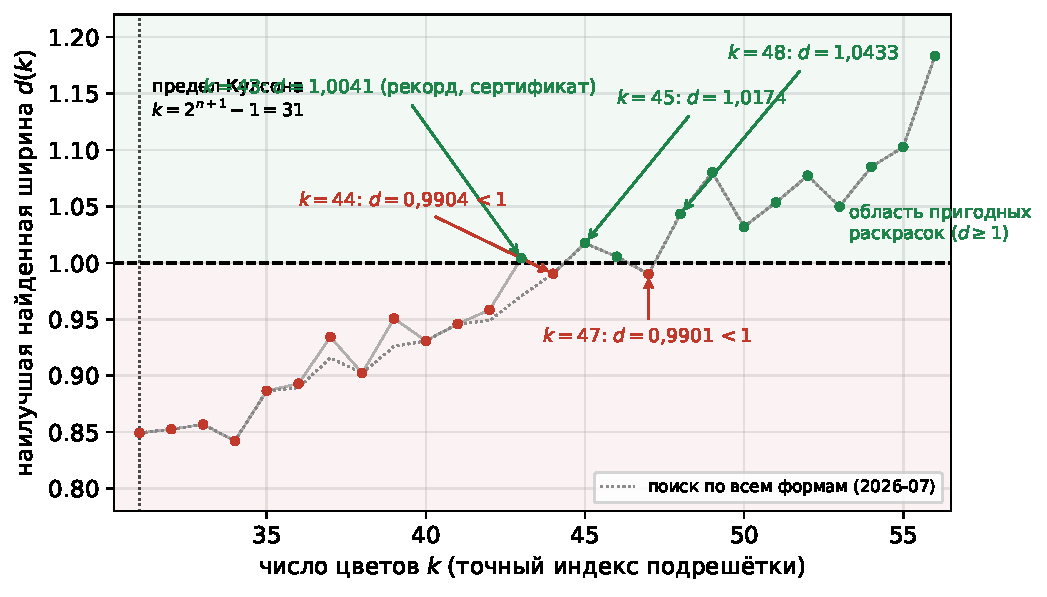
\includegraphics[width=0.74\textwidth]{fig_descent.pdf}
\caption{Наилучшая найденная нормированная ширина $d(k)$ при \emph{точном}
индексе подрешётки $k$ (оптимизация метрики по всем 4-мерным решёткам). Зелёные
точки ($d\ge1$) отвечают пригодным раскраскам, красные --- нет. Рекорд ---
индекс $45$: показан численный оптимум $d=1{,}0174$, тогда как точный сертификат
даёт для рациональной формы $d=1{,}016339$ (\S\ref{sec:comp}). Немонотонность (например,
провал при простом $k=47$) отражает теоретико-числовую структуру: число
доступных подрешёток зависит от разложения $k$ на множители, поэтому <<богатые>>
составные индексы ($45=3^2\!\cdot5$, $48=2^4\!\cdot3$) пробиваются легче.
Левая часть --- кампания <<ниже 45>>: все $31\le k\le44$ дают $d<1$
(максимум $0{,}990$ при $k=44$); пунктир --- предел Кулсона $k=31$.}
\label{fig:descent}
\end{figure}

\subsection{Численный оптимум}

Рациональная форма~\eqref{eq:gram} --- это <<огрубление>> (со знаменателями
$\le16$) точного численного оптимума задачи $\max_Q d(Q,45)$. Сам оптимум даёт
несколько большую ширину, $d=1{,}0174005\ldots$ (значение независимо
воспроизведено двумя реализациями конвейера), при той же матрице
перехода~\eqref{eq:hnf}. Для строгой формулировки теоремы~\ref{thm:main}
используется рациональная форма, допускающая точный сертификат.


\subsection{Точный сертификат неравенства $d>\ell_0$}\label{sec:comp}


Помимо согласия трёх независимых численных алгоритмов
(\S\ref{sec:algo}, пункт~3), неравенство $d>\ell_0=1{,}015$ для
формы~\eqref{eq:gram} проверено \emph{в точной рациональной арифметике}. Идея ---
заменить (недоступный в замкнутой форме) многогранник $V_0$ на объемлющий
многогранник $P\supseteq V_0$ с рациональными вершинами и оценивать всё через
него: $\diam V_0\le\diam P$ и $\dist(p,V_0)\ge\dist(p,P)$.

Пусть $P$ --- пересечение $30$ полупространств-биссекторов
$\{x:\langle x,v\rangle_Q\le\tfrac12\langle v,v\rangle_Q\}$ по $15$ парам
целочисленных релевантных векторов $\pm v$. Каждый биссектор содержит $V_0$,
поэтому $V_0\subseteq P$.
\begin{enumerate}[leftmargin=1.8em]
\item[(а)] \textbf{Диаметр сверху.} Все вершины $P$ перечислены точно (решение
$\binom{30}{4}=27\,405$ рациональных систем $4\times4$ с проверкой всех
неравенств; вершин ровно~$120$), откуда
$\diam^2 V_0\le\diam^2 P=\tfrac{3462746607825546397}{147660219970227360}
=23{,}450775087\ldots$
\item[(б)] \textbf{Расстояние снизу.} Для каждого вектора $v\in\Gamma_\star$ в
доказуемо полном окне~\eqref{eq:window}: либо точно $\langle v,v\rangle_Q\ge W^2$
с рациональным $W^2\ge(1+\ell_0)^2\diam^2P$ (тогда
$D(v)\ge\|v\|-\diam V_0\ge\ell_0\diam V_0$ автоматически), либо --- для $10$
коротких кандидатов --- применяется опорное неравенство
\[
\dist(v/2,P)\ \ge\
\frac{\langle v/2,u\rangle_Q-\max_{w\in\mathrm{vert}\,P}\langle w,u\rangle_Q}
{\|u\|_Q}
\]
с рациональным направлением $u$. Все величины --- точные дроби; в итоге
\[
D(\Gamma_\star)^2\ \ge\ \frac{8261571747025}{341057837637}=24{,}223374558\ldots
\]
\item[(в)] \textbf{Вывод.} $\ell_0^2\,\diam^2P=24{,}159574764\ldots$, и так как
$24{,}223374558>24{,}159574764$, получаем
$D(\Gamma_\star)^2>\ell_0^2\diam^2V_0$, то есть $d>\ell_0$ строго. \qed
\end{enumerate}
Плавающая арифметика используется лишь для \emph{выбора} кандидатов и направлений
$u$ (на строгость не влияющего). Дополнительно исчерпывающим перебором всех
$188\,760$ подрешёток индекса~$45$ подтверждено, что~\eqref{eq:hnf} доставляет
максимум $d$ для $\Lambda_\star$.


\section{Размерности 5 и 7: $\chi(\R^5)\le132$ и $\chi(\R^7)\le1323$}
\label{sec:r57}

В этих размерностях исчерпывающий перебор подрешёток недоступен, и обе
конструкции получены чередованием дискретного поиска ядра с непрерывной
деформацией формы Грама (\S\ref{sec:big}). Ниже сначала описано, как найдено
ядро, затем приведён точный сертификат.

\subsection{Спуск $140\to132$ в $\R^5$}

Прежняя оценка $140$ получена АБПР на решётке $A_5^*$, и там же доказана её
минимальность --- но лишь среди подрешёток \emph{этой} решётки. Наш спуск идёт
ступенями $140\to139\to136\to134\to133\to132$, и на каждой меняются и ядро, и
форма Грама. Первая ступень описана в \S\ref{sec:big} как иллюстрация
примарного шага; опишем остальные.

Для промежуточного результата $136$ проверены типы
$[17,8]$, $[17,4,2]$ и $[17,2,2,2]$. Тип $[17,8]$ после повторного обмена
геометрическими весами и деформации формы пересёк порог в двух независимых
стохастических продолжениях. Доводка по активному набору дала численный минимум
$1{,}0008145796$.

Локальный максимум при $134=67\cdot2$ удалось обойти так. Вместо ширины одного
ядра мы максимизировали вторую по величине из ширин двух ядер сразу: полученная
форма Грама хороша не для одного из них, а для обоих. На этой форме
исчерпывающий перебор с порогом $0{,}90$ дал $28$ новых пригодных ядер --- по
одному на каждую допустимую строку проективного пространства. Четыре лучших из этих ядер были независимо продолжены по метрике;
второе пересекло единицу уже на $97$-м поколении CMA-ES и дал
промежуточную доказанную оценку~$134$.

Затем на полученной форме были намеренно запущены поиски сразу при индексах
$133$, $132$ и $131$. Для $133$ две независимые деформации пересекли единицу.
Для $132$ блочные типы $[11,3,2,2]$ и $[11,3,4]$ дали три пересечения;
лучшее из них доводка по активному набору подняла с $1{,}003354222\ldots$ до
$1{,}010905284\ldots$. Это демонстрирует немонотонность качества соседних
арифметических типов: проверка сразу на два цвета ниже оказалась успешнее
остановки на первом пересечённом индексе. Именно конструкция индекса~$132$
рационализована ниже.

\begin{theorem}\label{thm:r5}
Существует решёточная раскраска
\[
 \chi\bigl(\R^5,[1,\ell]\bigr)\le132
 \qquad\text{для всех }\ell\le\frac{101}{100}.
\]
В частности, $\chi(\R^5)\le132$.
\end{theorem}

\begin{proof}[Компьютерно проверяемое доказательство]
Пусть $\Lambda=B^{\mathsf T}\Z^5$, где $BB^{\mathsf T}=Q$ и
\[
Q=\frac1{100000}
\begin{pmatrix}
79327&86284&69597&36140&26501\\
86284&254538&216808&101257&102135\\
69597&216808&296568&163667&140527\\
36140&101257&163667&181733&71653\\
26501&102135&140527&71653&148076
\end{pmatrix}.
\]
Её главные угловые миноры
\[
79327,\ 12746807270,\ 1422467480626358,\
124437401434750889345,\ 9999935596575703407615413
\]
положительны. Зададим цвет координатного вектора $x\in\Z^5$ тройкой
гомоморфизмов
\[
\begin{aligned}
\varphi_{11}(x)&=x_2+6x_3+2x_4+3x_5\pmod {11},\\
\varphi_3(x)&=x_1+2x_2+x_3\pmod 3,\\
\varphi_4(x)&=x_2+3x_3+x_4+3x_5\pmod 4.
\end{aligned}
\]
По китайской теореме об остатках это эквивалентно одной строке
\[
\varphi(x)=88x_1+89x_2+127x_3+57x_4+3x_5\pmod {132}.
\]
Положим $\Gamma=B^{\mathsf T}\ker\varphi$. Гомоморфизм сюръективен,
$[\Lambda:\Gamma]=132$, а Smith-диагональ ядра равна
$(1,1,1,1,132)$.

Ячейка Вороного рациональной формы $Q$ имеет $62$ фасеты и $720$ вершин.
Все вершинные системы решены над $\mathbb Q$; точный квадрат радиуса покрытия
равен
\[
R^2=
\frac{3093570095915736710467707313641}
     {3999974238630281363046165200000}.
\]
Доказываемое утверждение --- это $D(v)\ge\ell\,\diam V_0$ при $\ell=101/100$,
поэтому из $D(v)\ge\|v\|-\diam V_0=\|v\|-2R$ следует, что возможный нарушитель
обязан удовлетворять
\begin{equation}\label{eq:win5}
\|v\|<2(1+\ell)R,\qquad\text{т.е.}\qquad \|v\|^2<12{,}4985\ldots
\end{equation}
Отметим, что более узкое окно $\|v\|<4R$ отвечает лишь цели $d>1$ и для
интервального утверждения недостаточно. Перебор Финке--Поста по LLL-приведённому
базису $\Gamma$ оставляет в окне~\eqref{eq:win5} ровно $38$ ненулевых векторов
($19$ пар); из них $36$ лежат уже в окне $\|v\|<4R$ и независимо воспроизводятся
C\raise.1ex\hbox{\small++}-перечислителем, а оставшаяся пара
$\pm(-2,2,-2,2,2)$ даёт $D/\diam V_0=1{,}0442\ldots$ и на минимум не влияет.

Для всех $38$ векторов задача проекции на $V_0$ решена точно: допустимость,
неотрицательность множителей ККТ и значения целей проверены над $\mathbb Q$.
Минимум достигается на паре
$\pm(2,0,1,-3,0)$ (координаты по базису $\Lambda$) и равен
\[
\begin{aligned}
D_{\min}^2&=
\frac{1634114770527727}{516898614620000},\\
D_{\min}^2-\left(\frac{101}{100}\right)^2 4R^2
&=\frac{1450500657237822255902962097875907780124229}
{258447642807960215367421006872956903000000000}>0.
\end{aligned}
\]
Следовательно,
$D_{\min}/\diam V_0=1{,}010897714548927\ldots>1{,}01$.
Раскраска ячеек по классам $\Lambda/\Gamma$ даёт требуемые $132$ цвета.
Полный список вершинных инцидентностей и KKT-сертификатов, а также независимая
проверка множества из $1025$ пар $\pm v$, запрещённых при пороге $\ell=1$,
находятся в файле
\path{audit-data/hd-$2026$-07/metric_deform_a5_132_refined_certificate.json}.
Дополнительный верификатор, не использующий Qhull или вещественный
перечислитель коротких векторов, точно проверяет все $31$ ненулевых
класса чётности, строит $62$ фасеты, обходит связный граф из $720$ вершин и
$1800$ рёбер и воспроизводит те же $R^2$, $D_{\min}^2$ и KKT-сертификаты;
его протокол ---
\path{audit-data/hd-$2026$-07/metric_deform_a5_132_refined_independent_exact_audit.json}.
Наконец, весь независимый аудит повторён после рационализации той же численной
формы со знаменателями $10^4$ и $10^6$; получены отношения соответственно
$1{,}010770760\ldots$ и $1{,}010904642\ldots$, и в обоих случаях также
сохраняется строгий запас для $\ell=1{,}01$.
\end{proof}

\paragraph{Барьер $1372$ на фиксированной решётке $E_7^*$.} Для $\R^7$
\cite{ABPR} получили оценку $1372$ решёткой $E_7^*$ \emph{рандомизированным}
поиском, без доказательства минимальности (в отличие от $\R^5$, где минимальность
$140$ доказана полным перебором). Мы воспроизвели их конструкцию точно (матрицы
$M$, $C_7$ из \cite{ABPR}: $|F_1|=24\,284$, $|\det C_7|=1372$, $\Lambda'\cap
F=\varnothing$; отношение покрытие/упаковка $E_7^*$ равно $\sqrt{7/3}$) и
проверили её на понижение индекса. Подрешётка $C_7$ оказалась
\emph{неуплотняемой}: не существует \emph{надрешётки} $\Lambda''\supset\Lambda'$
индекса $1372/p$ ($p\in\{2,7\}$), избегающей $F$ (любой склеивающий вектор
порядка $p$ попадает в $F$). Ни градиентный спуск, ни отжиг, ни $2\cdot10^6$
случайных базисов из коротких незапрещённых векторов не дали пригодной подрешётки
индекса ${<}1372$ (случайные пригодные подрешётки встречаются лишь с индексом
${\ge}2052$). Это --- вычислительное свидетельство оптимальности $1372$ среди
раскрасок с фиксированной родительской решёткой $E_7^*$, но не среди всех форм
Грама.


\subsection{Спуск $1372\to1323$ в $\R^7$}

Прямые атаки на фиксированную $E_7^*$ упирались в барьер (см.\ выше), поэтому
здесь понадобились обе стадии сразу: примарный Radon-поиск ядра
(\S\ref{sec:big}) и последующая деформация формы Грама. При структуре
$(\Z/7)^2\times(\Z/3)^3$ поиск дал ядро индекса $1323$, у которого на
$E_7^*$ остаются лишь шесть конфликтов одинаковой тяжести
$D/\diam V_0=0{,}886405\ldots$. После этого ядро фиксируется, а родительский
базис деформируется как $B=B_0\exp H$, где $H=H^{\mathsf T}$ и
$\operatorname{tr}H=0$. В отличие от прежней целочисленной цели --- числа неотделённых векторов ---
непрерывной целью служит непосредственно $\min D/\diam V_0$.

\begin{theorem}\label{thm:r7}
Существует решёточная раскраска
\[
 \chi\bigl(\R^7,[1,\ell]\bigr)\le1323
 \qquad\text{для всех }\ell\le1{,}007.
\]
В частности, $\chi(\R^7)\le1323$.
\end{theorem}

\begin{proof}[Компьютерно проверяемое доказательство]
Пусть $\Lambda=B^{\mathsf T}\Z^7$, где $BB^{\mathsf T}=Q$ и
\[
\begingroup
\setlength{\arraycolsep}{2.6pt}
Q=\frac1{10\,000}\!
\begin{pmatrix}
20968&-10761&-529&-2493&6504&-6603&-796\\
-10761&22451&-9533&1398&-2933&1926&13148\\
-529&-9533&21640&-12309&-430&1476&-630\\
-2493&1398&-12309&22527&-9467&974&1288\\
6504&-2933&-430&-9467&18435&-11881&-1083\\
-6603&1926&1476&974&-11881&20755&-99\\
-796&13148&-630&1288&-1083&-99&18191
\end{pmatrix}.
\endgroup
\]
Все главные угловые миноры числителя положительны. Зададим
$\Gamma=B^{\mathsf T}C\Z^7$ матрицей
\[
\begingroup
\setlength{\arraycolsep}{3.2pt}
C=\begin{pmatrix}
21&0&9&17&16&14&2\\
0&21&9&0&10&14&20\\
0&0&3&1&1&2&0\\
0&0&0&1&0&0&0\\
0&0&0&0&1&0&0\\
0&0&0&0&0&1&0\\
0&0&0&0&0&0&1
\end{pmatrix}.
\endgroup
\]
Имеем $|\det C|=1323$, а нормальная форма Смита равна
$(1,1,1,1,3,21,21)$.

Для рациональной формы $Q$ ячейка Вороного имеет $254$ фасеты и является
простым многогранником с $39\,296$ вершинами. Все вершинные системы решены над
$\mathbb Q$; точный квадрат радиуса покрытия равен
\[
 R^2=
 \frac{42823481847474795123735510069131}
 {49956306567646383875936777960000}.
\]
Доказываемое утверждение --- это $D(v)\ge\ell\,\diam V_0$ при $\ell=1{,}007$,
поэтому из $D(v)\ge\|v\|-\diam V_0=\|v\|-2R$ следует, что возможный нарушитель
обязан удовлетворять
\begin{equation}\label{eq:win7}
 \|v\|<2(1+\ell)R,\qquad\text{т.е.}\qquad\|v\|^2<13{,}8117\ldots
\end{equation}
(более узкое окно $\|v\|<4R$ отвечало бы лишь цели $d>1$). Перебор Финке--Поста
по LLL-приведённому базису $\Gamma$ оставляет в окне~\eqref{eq:win7} ровно $72$
ненулевых вектора ($36$ пар); из них $70$ лежат уже в окне $\|v\|<4R$, а
оставшаяся пара $\pm(2,-1,0,0,0,0,1)$ даёт $D/\diam V_0=1{,}18905\ldots$ и на
минимум не влияет. Для каждого из них решена задача проекции на $V_0$,
причём допустимость, неотрицательность множителей ККТ и значение цели проверены
над $\mathbb Q$. Минимум достигается на паре
$\pm(1,0,0,2,1,0,1)$ (координаты по базису $\Lambda$) и равен
\[
 D_{\min}^2=\frac{21004929056}{6040637375},\qquad
 D_{\min}^2-\left(\tfrac{1007}{1000}\right)^2 4R^2>0,
\]
где последняя разность равна в точности
\[
 \frac{134661904230636621379975888187452316904519}
 {603535865138965424449162128164504510000000000}.
\]
Следовательно,
$D_{\min}/\diam V_0=1{,}007032309005\ldots>1{,}007$.
Раскрашивая ячейки Вороного по классам $\Lambda/\Gamma$, получаем требуемые
$1323$ цвета. Счётчики вершин и фасет, сертификаты ККТ и независимая проверка
$\ker\varphi\cap F=\varnothing$ находятся в файле
\path{audit-data/hd-$2026$-07/metric_deform_e7_1323_certificate.json}.
\end{proof}

\paragraph{Границы \emph{клеточных} раскрасок на фиксированной форме.}
Схема АБПР --- частный случай \emph{клеточной} раскраски (цвет
постоянен на внутренности ячейки Вороного). Общая клеточная раскраска с периодом
$\Gamma$ --- это правильная раскраска \emph{графа конфликтов} $H_\Gamma$ на
$\Lambda/\Gamma$ (метрический аналог раскраски графа касания ячеек Вороного
\cite{DSMMV}): вершины --- классы, ребро $[a]\!\sim\![b]$, если пара ячеек
реализует запрещённое расстояние. АБПР дают каждому классу свой цвет
($[\Lambda:\Lambda']$ цветов), но $\chi(H_\Gamma)$ \emph{в принципе} может быть
меньше. Мы установили, что здесь это не так.

\emph{(i) Граф не разрежается.} Множество рёбер \emph{точно} отвечает $F$:
для всякого $v\in F$ пара ячеек $V_0$ и $v+V_0$ действительно реализует
запрещённое расстояние, поскольку наряду с $D(v)<\diam V_0$ выполнено и
$D'(v)\ge2R$ для наибольшего расстояния $D'(v)$ между этими ячейками (проверено
перебором вершин).

\emph{(ii) При периоде $\Gamma=\Lambda'$ выигрыша нет.} Здесь $F$ покрывает
\emph{все} ненулевые классы $\Lambda/\Lambda'$ (проверено для $A_5^*/140$ и
$E_7^*/1372$), так что $H_{\Lambda'}$ --- полный граф
$K_{[\Lambda:\Lambda']}$ и $\chi(H_{\Lambda'})=[\Lambda:\Lambda']$.

\emph{(iii) Измельчение периода тоже не помогает.} Для проверенных
$\Gamma\subsetneq\Lambda'$ граф конфликтов оказывается полным многодольным; в
$\R^5$ при периоде индекса $280$ равенство $\chi(H_\Gamma)=140$ \emph{доказано}
SAT-решателем. Клика у этих измельчённых графов меньше индекса ($80$ в $\R^5$
и $541$ в $\R^7$), так что чисто кликовая нижняя оценка здесь недостаточна, --- и
тем не менее во всех опробованных случаях хроматическое число совпадало с
индексом. Эти отрицательные результаты относятся к фиксированным
симметричным родительским решёткам. Теорема~\ref{thm:r7} показывает, что
совместная смена ядра и формы Грама обходит барьер без перехода к
подъячеечным раскраскам. Строгое утверждение о клеточных раскрасках на
фиксированной $E_7^*$ остаётся открытым.


\section{Интервальные версии: более широкие запрещённые отрезки}
\label{sec:wide}

Метод даёт не только оценки на $\chi(\R^n)$, но и раскраски, запрещающие целый
отрезок расстояний. Здесь собраны такие результаты: компромисс
<<цвета\,$\leftrightarrow$\,ширина>> в $\R^4$, лестницы ширин в $\R^2$--$\R^6$ и
улучшения в $\R^3$.

\subsection{Более широкий интервал в $\R^4$: $\chi(\R^4,[1,\ell])\le48$}


При индексе~$48$ та же оптимизация даёт заметно большую ширину. Для рациональной
решётки с матрицей Грама
\[
Q_{48}=\begin{pmatrix}
\tfrac{137}{12}&\tfrac{13}{7}&-\tfrac{61}{10}&-\tfrac{18}{5}\\[2pt]
\tfrac{13}{7}&7&-\tfrac{25}{9}&-\tfrac{37}{12}\\[2pt]
-\tfrac{61}{10}&-\tfrac{25}{9}&12&-\tfrac{17}{11}\\[2pt]
-\tfrac{18}{5}&-\tfrac{37}{12}&-\tfrac{17}{11}&\tfrac{44}{5}
\end{pmatrix}
\]
и подрешётки индекса~$48$ с наддиагональю $(28,16,30)$ в последнем столбце
получается $d=1{,}039657681\ldots$ (здесь $\lambda_1^2=7$,
$\diam^2P=19{,}141641$, $D^2\ge20{,}689971$); тем же точным сертификатом
доказывается
\[
\chi\bigl(\R^4,[1,\ell]\bigr)\le48\qquad(\ell\le1{,}0396).
\]
Численный оптимум при индексе~$48$ достигает $d=1{,}0432696$. Итак, увеличив
число цветов на три ($45\to48$), можно заметно расширить запрещённый интервал
($1{,}015\to1{,}0396$) --- этот компромисс <<цвета${}\leftrightarrow{}$ширина>>
ранее не отмечался.

\subsection{Сводка результатов в $\R^4$}

Таблица~\ref{tab:r4} собирает все три полученные решёточные раскраски $\R^4$:
рекордную по числу цветов ($45$) и две с более широким запрещённым интервалом
($46$, $48$). Каждая задаётся рациональной решёткой общего положения (ячейка ---
пермутоэдр с $f$-вектором $(120,240,150,30)$) и подрешёткой с циклической
матрицей перехода; для каждой доказан точный сертификат $d>\ell_0$. Матрицы
Грама для $k=45$ и $k=48$ выписаны выше, для $k=46$ --- в файле
\path{audit-data/cert46.json}.

\begin{table}[h]
\centering
\caption{Полученные раскраски $\R^4$: $\chi(\R^4,[1,\ell])\le k$ при
$\ell\le\ell_0$. Столбец <<знам.>> --- наибольший знаменатель рациональной
матрицы Грама; <<$d$ (числ.)>> --- ширина численного оптимума.}
\label{tab:r4}
\small
\begin{tabular}{c c c c c l}
\toprule
$k$ & $\ell_0$ (сертиф.) & $d$ (рацион.) & $d$ (числ.) & знам. & примечание\\
\midrule
\textbf{45} & $\mathbf{1{,}015}$ & $1{,}016339$ & $1{,}017401$ & $16$
  & \textbf{рекорд по числу цветов}\\
46 & $1{,}004$ & $1{,}005069$ & $1{,}005405$ & $24$ & промежуточный\\
48 & $1{,}0396$ & $1{,}039658$ & $1{,}043270$ & $12$ & наибольший интервал\\
\bottomrule
\end{tabular}
\end{table}

\subsection{Лестницы ширин и улучшения в $\R^3$}\label{sec:stair}

Дешевизна оценки формы (\S\ref{sec:big}) позволяет строить \emph{лестницы ширин}
и в старших размерностях: при большем числе
цветов запрещённый интервал расширяется (на фиксированной $A_5^*$ до
$[1,\,1{,}265]$ при $k=300$, табл.~\ref{tab:stair56}). При $n\ge7$ запрещённое множество быстро растёт
($|F_1|\approx1{,}9\cdot10^4$ для $A_7^*$,
${\approx}3{,}5\cdot10^4$ для $E_7$), поэтому сплошной перебор индексов
становится дорогим и поиск ведётся по \emph{курируемым} индексам.


Рис.~\ref{fig:stair} показывает <<лестницы>> максимальной ширины $d(k)$ ---
бегущий максимум по классическим решёткам --- для $\R^2$, $\R^3$, $\R^4$. Порог
$d=1$ впервые достигается при $k=7$ (шестиугольная решётка, $\R^2$), $k=15$
(BCC, $\R^3$) и $k=49$ по классическим решёткам в $\R^4$ (генерические решётки
опускают его до~$45$, \S\ref{sec:main}).

\begin{figure}[t]
\centering
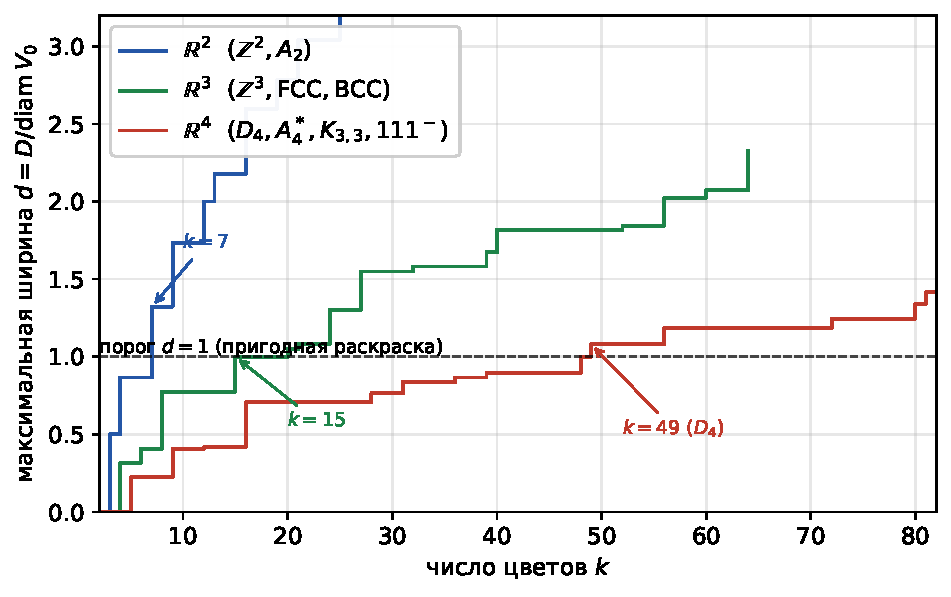
\includegraphics[width=0.74\textwidth]{fig_staircase.pdf}
\caption{Максимальная нормированная ширина $d(k)$ как функция числа цветов $k$
для $\R^2$, $\R^3$, $\R^4$ (бегущий максимум по классическим решёткам каждой
размерности). Пунктир --- порог $d=1$: правее точки пересечения раскраска в $k$
цветов правильна для классического расстояния.}
\label{fig:stair}
\end{figure}

(Здесь запись <<$\R^4$, $k=49$>> относится к классическим решёткам; выход в
генерические решётки даёт $46$, $48$ и рекордные $45$ цветов, \S\ref{sec:main}.)

\paragraph{Размерность 3: оптимальность 15 цветов и расширение интервала.}
В отличие от $\R^4$, в $\R^3$ число цветов уменьшить нельзя: нижняя граница
Кулсона для решёточных раскрасок $\chi_s\ge2^{n+1}-1$ \cite{Coulson,ABPR} даёт
$\chi_s(\R^3)\ge15$, и это подтверждается численно --- оптимизация метрики при
$k=8,\dots,14$ ни разу не достигает порога $d=1$ (максимум $d=0{,}900$ при
$k=14$). Значит $15$ цветов --- оптимум среди решёточных раскрасок $\R^3$.
Отметим, что у классического $15$-цветника на BCC ширина равна в точности
$d=1$, и предложение~\ref{prop:crit}, требующее \emph{строгого} неравенства
$\ell<d$, к нему неприменимо: оценка $\chi(\R^3)\le15$ получена Кулсоном
\cite{Coulson} отдельным разбором границ ячеек. Наш результат этой тонкости не
требует: \emph{интервальную} версию можно улучшить уже при $15$ цветах, причём
со строгим запасом --- генерическая решётка даёт $d=1{,}0266$, т.е.
\[
\chi\bigl(\R^3,[1,\ell]\bigr)\le15\qquad(\ell\le1{,}0266),
\]
--- целый запрещённый интервал вместо единственного расстояния у BCC.

При $k>15$ оптимизация метрики по всему пространству форм заметно улучшает
нашу прежнюю таблицу \cite{Ivanov2011} для $\R^3$ (табл.~\ref{tab:r3}; каждое значение
--- явная решётка и подрешётка): при $k=21,23,24$ ширины существенно больше, а
для многих $k$ (в т.ч. пороговый $k=15$) оценки получены впервые.

\begin{table}[h]
\centering
\caption{Ширина $d$ запрещённого интервала для $\chi(\R^3,[1,\ell])\le k$ при
оптимизации метрики по всему пространству квадратичных форм (выборка $k$).
Прочерк --- значение, отсутствующее в \cite{Ivanov2011}.}
\label{tab:r3}
\small
\begin{tabular}{c cccccccccc}
\toprule
$k$ & 15 & 18 & 20 & 21 & 23 & 24 & 27 & 32 & 40 & 49\\
\midrule
$d$ (наст. раб.) & $\mathbf{1{,}027}$ & $1{,}116$ & $1{,}172$ & $\mathbf{1{,}263}$
  & $\mathbf{1{,}253}$ & $\mathbf{1{,}364}$ & $1{,}549$ & $1{,}581$ & $1{,}822$
  & $1{,}914$\\
$d$ (\cite{Ivanov2011}) & --- & $1{,}116$ & --- & $1{,}134$ & $1{,}137$ &
  $1{,}304$ & $1{,}549$ & --- & --- & ---\\
\bottomrule
\end{tabular}
\end{table}

\noindent Попутно исправлены три опечатки, допущенные в матрицах подрешёток
в~\cite{Ivanov2011}. Верные матрицы таковы: для $\R^3$ при $k=21$ ---
диагональ $(3,1,7)$ с наддиагональю $(0,0,5)$; для разрежённой серии при $k=14$
--- наддиагонали $(0,0,12)$ и $(0,0,10)$.

\paragraph{Размерности 5 и 6: лестницы на $A_5^*$ и $E_6^*$.} Дешёвая оценка
формы (\S\ref{sec:big}) впервые позволяет проследить лестницу ширин и в старших
размерностях. Для $\R^5$ подрешётки решётки $A_5^*$ различных индексов дают
расширяющийся запрещённый интервал (табл.~\ref{tab:stair56}): порог $d=1$
на \emph{фиксированной} $A_5^*$ достигается при $k=140$ (конструкция $C_5$,
$d=\sqrt{39/35}$), а уже при
$k=196,270,300$ ширина растёт до $\sqrt{7/5},\ \sqrt{54/35},\ \sqrt{8/5}$ ---
интервальные оценки $\chi(\R^5,[1,\ell])\le k$, ранее не отмечавшиеся. В $\R^6$
метод воспроизводит эйзенштейнову подрешётку $E_6^*/343$ с точной шириной
$\sqrt{7/6}$ (\S\ref{sec:extra}) как \emph{минимальный} по числу цветов
решёточный порог. Раскраски найдены масштабируемым поиском
(\S\ref{sec:big}); нормированные ширины вычислены как $\min_{v\in\Gamma\setminus0}
D(v)/\diam V_0$ и совпадают с указанными рациональными $d^2$ до $5$ знаков.

\begin{table}[h]
\centering
\caption{Лестница ширин запрещённого интервала в $\R^5$ (решётка $A_5^*$) и
опорная точка в $\R^6$ (решётка $E_6^*$): $\chi(\R^n,[1,\ell])\le k$ при
$\ell<d$. Строка $k=140$ совпадает с точным результатом АБПР (табл.~в
\S\ref{sec:extra}); новая конструкция индекса 132 использует другую форму и
приведена в теореме~\ref{thm:r5}.}
\label{tab:stair56}
\small
\begin{tabular}{c c l l l}
\toprule
$n$ & $k$ & решётка & $d^2$ & $d$\\
\midrule
5 & 140 & $A_5^*$ & $39/35$ & $1{,}0556$\\
5 & 196 & $A_5^*$ & $7/5$   & $1{,}1832$\\
5 & 270 & $A_5^*$ & $54/35$ & $1{,}2421$\\
5 & 300 & $A_5^*$ & $8/5$   & $1{,}2649$\\
6 & 343 & $(3+\omega)E_6^*$ & $7/6$ & $1{,}0801$\\
\bottomrule
\end{tabular}
\end{table}


\section{Полная картина: точные ширины конструкций АБПР}\label{sec:extra}

Метод применим и как <<измерительный инструмент>>: для каждой явной решёточной
конструкции из \cite{ABPR} можно вычислить точную ширину $d$ её запрещённого
интервала (в самой работе доказывалось лишь $d\ge1$). Добавим к ним новые
рациональные конструкции настоящей работы. Результаты для $4\le n\le9$
(каждая строка --- оценка $\chi(\R^n,[1,\ell])\le k$ при $\ell<d$):

\begin{center}\small
\begin{tabular}{c c l l l}
\toprule
$n$ & $k$ & решётка / конструкция & $d^2$ & $d$\\
\midrule
4 & 45   & $\Lambda_\star$ (наст. работа) & --- & $1{,}016339$\\
4 & 48   & (наст. работа, \S\ref{sec:wide}) & --- & $1{,}039658$\\
4 & 49   & $(3+\omega)D_4$ & $7/6$ & $1{,}080123$\\
4 & 54   & $A_4^*$ & $23/20$ & $1{,}072381$\\
5 & 132  & рациональная решётка общего положения (теорема~\ref{thm:r5})
  & --- & $1{,}010898$\\
5 & 140  & $A_5^*$, матрица $C_5$ из \cite{ABPR} & $39/35$ & $1{,}055597$\\
6 & 343  & $(3+\omega)E_6^*$ & $7/6$ & $1{,}080123$\\
7 & 1323 & рациональная решётка общего положения (теорема~\ref{thm:r7})
  & --- & $1{,}007032$\\
7 & 1372 & $E_7^*$, матрица $C_7$ из \cite{ABPR} & $17/14$ & $1{,}101946$\\
8 & 2401 & $(3+\omega)E_8$ & $7/6$ & $1{,}080123$\\
9 & 17253& $A_9^*$, матрица $C_9$ из \cite{ABPR} & $169/165$ & $1{,}012048$\\
\bottomrule
\end{tabular}
\end{center}

\paragraph{Тождество для эйзенштейновых конструкций.} Для решёток с
$\Z[\omega]$-структурой ($\omega=e^{2\pi i/3}$) и подрешётки
$\Gamma=(3+\omega)\Lambda$ (умножение на $\alpha=3+\omega$, $|\alpha|^2=7$) во
всех проверенных случаях ($n=2,4,6,8$) выполняется точное равенство
\begin{equation}\label{eq:eis}
D\bigl((3+\omega)\Lambda\bigr)^2=\tfrac73\,\lambda_1(\Lambda)^2,
\qquad\text{т.е.}\qquad
d=\frac{\sqrt{7/3}}{\,2R/\lambda_1\,},
\end{equation}
где $R$ --- радиус покрытия. Ширина $d$ зависит \emph{только} от отношения
покрытие/упаковка (рис.~\ref{fig:eis}): при $2R/\lambda_1=\sqrt2$ (решётки
$D_4$, $E_6^*$, $E_8$) получается ровно $d=\sqrt{7/6}$.

Подчеркнём, что сама пороговая константа $\sqrt{7/3}$ здесь не нова: в
замечании~9 работы \cite{ABPR} отмечено, что теорема~3 остаётся верной при
ослабленном условии $2R/\lambda_1\le\sqrt{7/3}\approx1{,}5275$ вместо $3/2$,
но авторы <<не знают решёток, которые использовали бы это усиление>>. Условие
$d\ge1$ в~\eqref{eq:eis} --- это в точности их ослабленное условие; новизна
здесь в другом: равенство~\eqref{eq:eis} даёт не только порог, но и \emph{точную}
ширину интервала для каждой конкретной решётки, а таблица выше как раз и
предъявляет решётки, реализующие усиление.

У решётки Лича $\Lambda_{24}$ отношение $2R/\lambda_1$ также равно $\sqrt2$;
в предположении, что~\eqref{eq:eis} сохраняется при $n=24$ (мы это не проверяли),
отсюда следовала бы гипотетическая оценка
$\chi\bigl(\R^{24},[1,\sqrt{7/6}]\bigr)\le7^{12}$. Для решётки Кокстера--Тодда
$K_{12}$ имеем $2R/\lambda_1=\sqrt{8/3}\approx1{,}633>\sqrt{7/3}$, и
формула~\eqref{eq:eis} даёт $d=\sqrt{7/8}\approx0{,}935<1$ --- конструкция
теоремы~3 из \cite{ABPR} на $K_{12}$ не проходит даже в усиленной форме
замечания~9 (частичный отрицательный ответ на их открытый вопрос~2).

\begin{figure}[t]
\centering
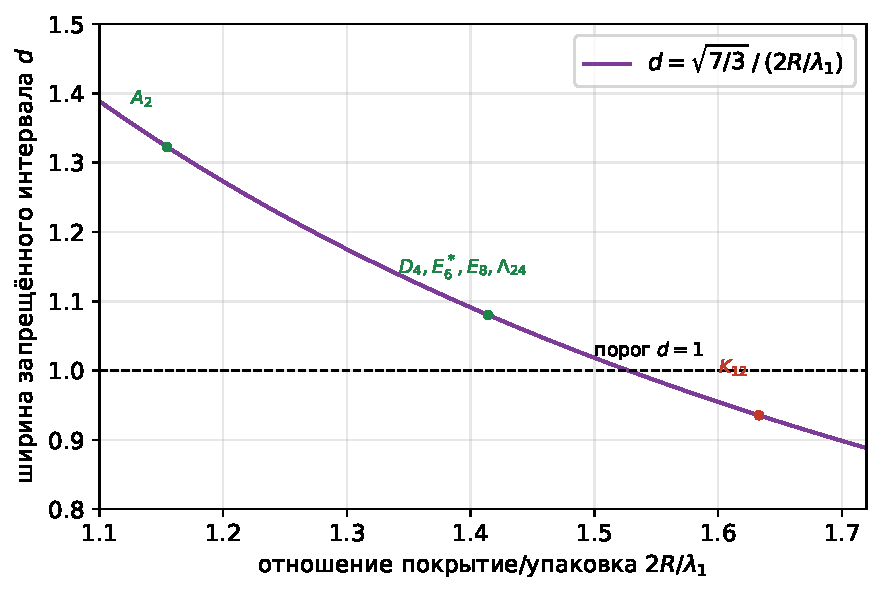
\includegraphics[width=0.6\textwidth]{fig_eisenstein.pdf}
\caption{Тождество~\eqref{eq:eis}: ширина $d$ эйзенштейновой конструкции против
отношения покрытие/упаковка $2R/\lambda_1$. Проверенные решётки $D_4,E_6^*,E_8$
(все с отношением $\sqrt2$) дают ровно $d=\sqrt{7/6}$; для $\Lambda_{24}$
положение точки предсказано в предположении~\eqref{eq:eis}, а для $K_{12}$
ширина падает ниже порога.}
\label{fig:eis}
\end{figure}

\paragraph{Оптимальность конструкции $C_5$ на фиксированной $A_5^*$.}
Исчерпывающим перебором \emph{всех} $1\,424\,115\,231$ подрешёток
индекса~$140$ решётки $A_5^*$ установлено, что явная конструкция $C_5$ из
\cite{ABPR} оптимальна на этом индексе и по ширине:
$\max d=\sqrt{39/35}$. Теорема~\ref{thm:r5} этому не противоречит: она меняет
родительскую форму и использует индекс~$132$.


\section{Границы метода и открытые вопросы}\label{sec:open}

\begin{enumerate}[leftmargin=1.5em]
\item \textbf{Насколько мал минимальный индекс?} Оптимизация метрики пробивает
порог $d=1$ вплоть до индекса~$45$ (с запасом $1{,}7\%$). Ниже целевая кампания
порога не пробила: при $k=44$ CMA-ES по формам Грама (восемь независимых
инстансов $\times\,2200$ точных оценок) и последующие мультистарты
Нелдера--Мида от найденных оптимумов выходят на плато $d=0{,}990$, а вдоль
лестницы $k=43,\dots,31$ наилучшая найденная ширина падает с $0{,}971$ до
$0{,}849$, хотя и немонотонно (рис.~\ref{fig:descent}). Дополнительно, для
проверенных пар <<решётка\,--\,структура факторгруппы>> при $36\le k\le44$
минимум числа неотделённых запрещённых векторов равен~$1$, а при $k=31$ и
$k=33$ --- от $1$ до $3$; заметим, что перебор структур здесь не был
исчерпывающим. Блокирующий вектор при этом не уникален и лежит глубоко в
запрещённом множестве, т.е.\ препятствие носит покрывающий, а не пороговый
характер.

Само по себе всё это \emph{не} является свидетельством невозможности: ровно ту
же сигнатуру --- ровно один неотделённый вектор --- прежняя бинарная цель давала
при $k=139$ в $\R^5$, а порог там был впоследствии пройден вплоть до $k=132$
(теорема~\ref{thm:r5}). Мы поэтому формулируем результат осторожно: спуск ниже
$45$ не удался ни одним из опробованных механизмов, но доказательства
минимальности у нас нет. Нижняя граница Кулсона $\chi_s\ge2^{n+1}-1=31$
\cite{Coulson,ABPR} формального препятствия к спуску не даёт; строгое
доказательство минимальности (или неожиданная конструкция с $31\le k\le44$) ---
открытая задача в духе вопроса~1 из \cite{ABPR}.
\item \textbf{Аналитическое описание.} Найти замкнутую форму оптимальных
генерических решёток для индексов $45$ и $48$ (предельных точек максимизации
$d$).
\item \textbf{Размерность 5: ниже $132$.} Предел Кулсона здесь равен $63$, то
есть формального препятствия к дальнейшему спуску нет. Тот же трёхшаговый
механизм (полный поиск ядра, деформация формы, доводка по активному набору),
применённый к индексам $131$, $130$ и $129$, порога не пересёк: лучшие
отношения равны соответственно $0{,}990216$, $0{,}976688$ и
$0{,}957014$~\textbf{[Э]}. Для каждого из них исчерпывающий конечнополевой
оракул подтвердил, что это глобальный дискретный максимум \emph{на
соответствующей фиксированной численной форме}; подробности ---
приложение~\ref{app:d5}.

\item \textbf{Размерность 6: оценка $343$ не улучшена.} Предел Кулсона
равен~$127$. Мы проверили как ближайшие индексы, так и арифметически
согласованные цели; ни один не достиг порога~\textbf{[Э]}:

\smallskip
\begin{center}\small
\begin{tabular}{c l l}
\toprule
$k$ & структура факторгруппы & лучшее $D/\diam V_0$\\
\midrule
$342=19\cdot3\cdot3\cdot2$ & циклическая / нециклическая & $0{,}940393$ / $0{,}924370$\\
$341$ & --- & ${\approx}\,0{,}9164$\\
$340=17\cdot5\cdot2\cdot2$ & нециклическая & $0{,}935190$ / $0{,}928955$\\
$338=13\cdot13\cdot2$ & нециклическая & $0{,}908895$\\
$333=37\cdot3\cdot3$ & нециклическая & $0{,}961088$\\
$329$, $322$, $315$ & сохраняют исх. характер & $0{,}944303$, $0{,}949097$, $0{,}933317$\\
$\mathbf{336=7\cdot4\cdot4\cdot3}$ & Smith $(1,1,1,1,4,84)$ & $\mathbf{0{,}984244}$\\
\bottomrule
\end{tabular}
\end{center}
\smallskip

Наиболее перспективна не ближайшая, а арифметически согласованная цель $336$:
фактор точной конструкции $343$ имеет Smith-тип $(1,1,1,7,7,7)$, и, сохранив
один исходный характер над $\mathbb F_7$, мы ищем три остаточных блока
совместно с формой. Точный переход через стены L-типа, последовательный SDP с отсекающими плоскостями и внешняя аппроксимация конуса линейными сечениями довели
отношение до $0{,}984244122$, то есть разрыв до порога сократился с $1{,}934\%$
до $1{,}576\%$. Три независимых подхода упираются в один и тот же барьер, что
указывает на исчерпанность текущего вторичного конуса: дальше нужно менять сам
конус, согласуя выбор периода с выбором формы. Проверены также раскраски, не
являющиеся раскрасками по классам смежности (периодические подъёмы, графы Кэли
конечного тора, аффинные семьи); ни одна не дала раскраску. Все детали ---
приложение~\ref{app:d6}.

\item \textbf{Размерность 7.} Примарный Radon-поиск и деформация формы понизили
оценку АБПР с $1372$ до $1323$ (теорема~\ref{thm:r7}), хотя все прямые атаки на
фиксированную $E_7^*$ давали барьер. Индексы $1322$, $1321$ и $1320$ проверены
как шаги $-1,-2,-3$; лучший дискретно-непрерывный фронтир получен при $1320$
и равен $0{,}975568590$. Повторный локальный поиск ядра на этой форме
воспроизвёл исходное ядро, но порог не пересёк. Следующие задачи --- продолжить
из нескольких ядер и добавить совместный штраф доверительной области. Разрыв с нижней
границей всё ещё огромен: $16\le\chi(\R^7)\le1323$.
\item \textbf{Размерности 8 и 9.} Ближайшие экраны при $2400$ (для $E_8$) и
$17\,250$ (для $A_9^*$) дают лишь $0{,}70710678$ и $0{,}825837653$~\textbf{[Э]};
оценки $2401$ и $17\,253$ не изменяются. Smith-структура
$\operatorname{diag}(1^4,7^4)$ объясняет, почему малые поправки здесь особенно
неэффективны: возмущение ранга меньше четырёх меняет определитель на число,
кратное~$7$, и потому не может дать $2400=2401-1$. Детали и найденная в
\cite{ABPR} смена координат для $C_9$ --- приложение~\ref{app:d89}.

\item \textbf{Тождество~\eqref{eq:eis}.} Доказать
$D((3+\omega)\Lambda)^2=\tfrac73\lambda_1^2$ для всех эйзенштейновых решёток или
описать область его справедливости.
\end{enumerate}


% Раздел о происхождении результатов, воспроизводимости и роли ИИ.
\section{Происхождение результатов, воспроизводимость и роль ИИ}
\label{sec:origin}

Работа сочетает доказательства, точные компьютерные сертификаты и обширный
численный поиск. Чтобы читатель не восстанавливал статус каждого утверждения по
контексту, ниже явно описаны шкала статусов, состав программного обеспечения,
проведённые независимые проверки и использование систем искусственного
интеллекта.

\subsection{Статусы утверждений}

Шкала \textbf{[Т]}\,/\,\textbf{[С]}\,/\,\textbf{[Ч]}\,/\,\textbf{[Э]} (с
модификатором \textbf{[Ч]}${}^{*}$ для кандидатов без сертификата диаметра)
введена в \S\ref{sec:intro}; уточним, что к чему относится. Статус \textbf{[Т]} имеют
предложение~\ref{prop:crit}, леммы~\ref{lem:sym} и~\ref{lem:mid}, планарная
теорема (предложение~\ref{prop:planar}), правило вещественного множителя
(предложение~\ref{prop:mult}), инрадиусная лемма~\ref{lem:inradius} со
следствием~\ref{cor:no-subgroup}, обе леммы о ламинировании
(\ref{lem:P1} и~\ref{lem:P2}), оба
экрана индекса (предложения~\ref{prop:mink} и~\ref{prop:inrfloor}),
продуктовое исчисление (предложение~\ref{prop:product}) вместе с
теоремой~\ref{thm:dim10} об оценке $45619$ и её следствиями для $\R^{25}$
и~$\R^{26}$, и пол мозаичного
принципа (теорема~\ref{thm:floor}). Равенство в тождестве~\eqref{eq:eis} для
конкретных решёток ($A_2$, $D_4$, $E_6^*$, $E_8$) установлено \emph{точными
вычислениями} и потому имеет статус \textbf{[С]}; нижняя граница <<$\ge$>>
доказана для всех эйзенштейновых решёток и имеет статус \textbf{[Т]}. Статус
\textbf{[С]} --- теоремы~\ref{thm:main},~\ref{thm:r5},~\ref{thm:r7} вместе с
сертификатом \S\ref{sec:comp}, сопутствующие конструкции индексов $46$ и~$48$
(\S\ref{sec:wide}), мозаичные ступени \S\ref{ssec:quant} и
интервальная ступень $\R^3/15$ (\S\ref{sec:stair}): каждая
сведена к конечному списку неравенств между явно выписанными дробями, так что
результат не зависит от корректности оптимизирующего кода --- достаточно
доверять программе, проверяющей этот список. Статус \textbf{[Ч]} имеют все
<<численные оптимумы>> в таблицах и оценки, опирающиеся на кусочные
сертификаты диаметра ($1029$, $7203$, $9604$, $28812$ и ширины ламинирований:
плавающая точка сведена к значениям явных квадратик в вершинах явных
политопов, но рациональная запись ещё не выполнена); модификатор
\textbf{[Ч]}${}^{*}$ несёт кандидат $21609$ (\S\ref{ssec:dim10lam}), чей
сертификат формально проходит, но с запасом на грани разрешения плавающей
точки. Статус \textbf{[Э]} ---
все отрицательные экраны: \S\ref{ssec:dim912neg}, \S\ref{sec:open} и
приложение~\ref{app:screens}.

Насколько существенна разница между \textbf{[С]} и \textbf{[Э]}, показывает
история индекса~$134$ в \S\ref{app:d5}: тамошний барьер был обойдён не
уточнением той же формы, а переходом к другой. Оценки $45$, $132$ и $1323$ не
опираются на \textbf{[Ч]} и \textbf{[Э]}; оценки $1029$, $7203$ и $28812$
имеют статус \textbf{[Ч]} указанной повышенной пробы.

\subsection{Программное обеспечение и данные}

Весь код и все промежуточные данные открыты:
\begin{center}
\url{https://github.com/ivaleo/Chromatic}\quad (лицензия MIT)
\end{center}

Репозиторий состоит из трёх пакетов и каталога данных:
\begin{itemize}[leftmargin=1.4em,itemsep=1pt]
\item \texttt{voronoi4d} (каталог \texttt{voronoi/}) --- эталонная реализация на
Python: построение ячейки Вороного, расстояние точка\,--\,многогранник каскадом
проекций, точная рациональная сертификация;
\item \texttt{combigeo} --- быстрое ядро на C\raise.1ex\hbox{\small++}
(перечисление коротких векторов методом Финке--Похста, GJK, локальный поиск
\texttt{min\_conflicts}, безвершинный радиус покрытия) с привязками к Python;
\item \texttt{chromatic} --- над-пакет, выполняющий перекрёстную сверку двух
независимых бэкендов (\texttt{compare\_backends});
\item \texttt{audit-data/} --- сертификаты, протоколы независимых аудитов и
результаты всех кампаний (${\sim}220$ файлов JSON, около $60$\,МБ), а также
\texttt{audit-data/chromatic\_research/} --- $125$ скриптов поисковых кампаний
в размерностях $2$--$26$, которыми получены результаты \S\ref{sec:big},
\S\ref{sec:dim912}--\ref{sec:tilings} и \S\ref{sec:open}.
\end{itemize}

Совокупный объём --- около $51\,000$ строк Python и $3\,400$ строк
C\raise.1ex\hbox{\small++}. Каждый сертификат содержит данные, достаточные для
независимой перепроверки без обращения к коду проекта: рациональную форму Грама,
матрицу подрешётки, точный квадрат радиуса покрытия, полный список
потенциально опасных векторов и KKT-сертификат проекции для каждого из них.

\subsection{Независимые проверки}

Ключевые величины проверялись не одним, а несколькими несовпадающими путями.

\begin{itemize}[leftmargin=1.4em,itemsep=2pt]
\item \emph{Две независимые реализации.} Расстояние
$\dist(v/2,V_0)$ вычисляется каскадом ортогональных проекций
(\texttt{voronoi4d}), алгоритмом GJK и решением задачи квадратичного
программирования (\texttt{combigeo}); на всех тестах три способа совпадают до
девяти значащих цифр.

\item \emph{Аудит без Qhull.} Для конструкции индекса~$132$ ячейка Вороного
строится повторно программой, не использующей ни Qhull, ни вещественный
перечислитель коротких векторов: она заново находит $31$ ненулевой
parity-класс, $62$ фасеты, обходит граф из $720$ вершин и $1800$ рёбер и
воспроизводит те же $R^2$, $D_{\min}^2$ и все KKT-сертификаты.

\item \emph{Устойчивость к рационализации.} Та же численная форма
рационализована с разными знаменателями ($10^4$, $10^5$, $10^6$): отношение
меняется в четвёртом знаке после запятой ($1{,}010771$, $1{,}010898$,
$1{,}010905$), и во всех трёх случаях строгий запас для $\ell=1{,}01$
сохраняется.

\item \emph{Повторная сертификация с нуля.} Все три \textbf{[С]}-сертификата
(индексы $45$, $132$ и $1323$) были заново воспроизведены программами, не
разделяющими с основным конвейером ни строчки кода: независимо найдены релевантные векторы, перечислены вершины ячейки
($120$, $720$ и $39\,296$), вычислен точный радиус покрытия и проверены все
KKT-сертификаты проекций; итоговые дроби совпали посимвольно. Эта
перепроверка выполнена в отдельной сессии с ИИ-ассистентом (аудит от
05.08.2026, протокол --- \texttt{journal/AUDIT-2026-08-05.md}), поэтому
независимость здесь означает независимость \emph{кода}, а не независимость
исполнителя.

\item \emph{Контроль геометрии.} Корректность построенной ячейки проверяется
соотношением Эйлера для $f$-вектора, центральной симметрией множества вершин и
равенством объёма определителю решётки. Полнота перечисления вершин
дополнительно контролируется тождеством
$\sum_{\text{вершины}}|\det(v_1,\dots,v_n)|=(n+1)!$, где $v_i$ --- релевантные
векторы активных фасет: сумма нормированных объёмов симплексов Делоне,
инцидентных узлу решётки, не зависит от комбинаторного типа ячейки.
\end{itemize}

\subsection{Использование систем искусственного интеллекта}

Работа выполнена с систематическим использованием ИИ-ассистента: вычислительный
конвейер, скрипты поисковых кампаний, иллюстрации и первоначальные редакции
текста статьи создавались в диалоговых сессиях с ним. Использовались
современные большие языковые модели общего назначения в агентной оболочке для
работы с кодом; конкретные версии менялись за время работы. Это зафиксировано
в истории репозитория: все коммиты, кроме двух ранних (\texttt{ad9279c} и
\texttt{9307135}), созданных тем же способом, несут трейлеры
\texttt{Co-Authored-By} с указанием использованной модели и идентификатора
сессии.

Конкретно с помощью ИИ-ассистента выполнены:
\begin{itemize}[leftmargin=1.4em,itemsep=1pt]
\item реализация всех алгоритмов (\S\ref{sec:algo}), включая ядро на
C\raise.1ex\hbox{\small++} и точные рациональные сертификаторы;
\item планирование, запуск и сопровождение длительных вычислительных кампаний,
в том числе исчерпывающих переборов объёмом до $2\cdot10^9$ конфигураций;
\item построение иллюстраций из данных экспериментов;
\item подготовка редакций текста статьи и сопроводительной документации.
\end{itemize}

Математическая рамка работы принадлежит не ИИ: метод раскраски по решёткам
Вороного и лемма о середине восходят к Иванову~\cite{Ivanov2011}, конструкции и
оценки-ориентиры $49$, $140$, $343$, $1372$, $2401$, $17\,253$ --- к Арману,
Бондаренко, Прымаку и Радченко~\cite{ABPR}, глобальный оптимизатор Q-поиска ---
к~А.~Горнову~\cite{GornovQ} (порт выполнен с исходного текста
первоисточника). Разделение вкладов внутри самого диалога таково: постановки
задач, направление поиска, критерии отбора и итоговая проверка результатов
принадлежат автору; конкретные механизмы --- выход в решётки общего
положения, CSP-переформулировка, примарный Radon-поиск, чередование ядра и
формы Грама, ламинирование, продуктовое исчисление ширин --- возникали в ходе
диалога с ассистентом и принимались или отбрасывались автором.

\paragraph{Что это меняет для читателя.} Для математической проверяемости
теорем --- ничего, и в этом смысл выбранной схемы работы: происхождение
поискового кода несущественно после того, как полный сертификат независимо
проверен. Оценки со статусом \textbf{[С]} сведены к конечным спискам
неравенств между явно выписанными рациональными числами; такой список
проверяется программой в несколько десятков строк, не имеющей ничего общего с
кодом, которым он получен, и его корректность не зависит ни от надёжности
оптимизирующего кода, ни от того, кем или чем этот код написан. Численные
результаты \textbf{[Ч]} и отрицательные экраны \textbf{[Э]} такой гарантии не
имеют и приводятся именно как эвристические ориентиры.

Ответственность за все утверждения, включая формулировки, полученные с помощью
ИИ-ассистента, несёт автор.


\appendix

\section{Отрицательные экраны в размерностях 5--9}\label{app:screens}

Здесь собраны подробности вычислительных кампаний, итоги которых приведены в
\S\ref{sec:open}. Все результаты этого приложения имеют статус \textbf{[Э]}:
это переборы, завершившиеся отрицательно на \emph{фиксированных} численных
формах. Они показывают, где остановились опробованные механизмы, но не
являются доказательствами невозможности --- см. случай индекса~$134$ ниже,
где такой барьер был обойдён сменой формы.

\subsection{Размерность 5: спуск до 132 и экраны ниже}\label{app:d5}

В $\R^5$ блочный поиск, расширение портфеля и чередование ядра с метрикой
понижают оценку АБПР с $140$ до $132$ (теорема~\ref{thm:r5}), хотя однократная
CMA-ES с бинарной целью всегда останавливалась на одном конфликте.
Индексы $139$, $136$ и $134$ были промежуточными доказанными результатами.

Специализированный конечнополевой оракул усиливает эти эвристические экраны:
после фиксации численной метрики каждая строка блока заменяется битовой маской
плохих векторов, а их произведение исчерпывается точно. Для $135$ при пороге
$0{,}978056$ проверено $1\,547\,170\,372$ набора блоков трёх типов;
для $134$ при $0{,}991322$ --- $634\,149\,671$ набор; для $133$ при
$0{,}96619$ --- $385\,308\,361$ набор: во всех случаях получена невыполнимость.
Контрольные пороги непосредственно ниже найденных значений восстанавливают
исходные ядра. На финальной численной форме промежуточной конструкции
индекса~$136$ были также исчерпаны $2\,082\,485\,047$ наборов блоков.
Смешанные блоки одной простой характеристики здесь могут перечисляться с
избытком; невыполнимость над таким надмножеством остаётся корректной. Таким образом,
дискретная оптимальность на каждой из этих \emph{фиксированных} форм проверена
глобально с точностью порядка $10^{-6}$.
Само множество плохих векторов здесь построено по метрике с плавающей точкой, поэтому это
не доказательство невозможности после изменения формы и не заменяет
рациональный сертификат теоремы. Действительно, прежний локальный потолок
$0{,}995366$ для индекса~$134$ был обойдён не шлифовкой той же формы, а
пороговым расширением портфеля на мостовой метрике: из $28$ новых точных
ядер один новый бассейн дал сертифицированное отношение
$1{,}010646405\ldots$ для промежуточного индекса~$134$. Затем прямые проверки
на один, два и три цвета ниже дали численные пересечения и для $133$, и для
$132$; последний рационализован с отношением
$1{,}010897714\ldots$. Этот пример показывает, почему невыполнимость на фиксированной метрике нельзя интерпретировать как глобальную невозможность и почему нельзя
останавливаться после проверки только $k-1$.

После сертификации 132 новый трёхшаговый экран был повторён уже относительно
этого рубежа. Для индекса~131 полный перебор всех значений с $10\,000$ рестартов,
повторный поиск на 132-метрике, деформации и доводка по активному набору сначала дали
$0{,}987424118$. Полный конечнополевой оракул затем исчерпал все
\[
 |\mathbb P^4(\mathbb F_{131})|
 =1+131+131^2+131^3+131^4=296\,765\,305
\]
проективных строк и подтвердил, что это глобальный дискретный максимум на
той фиксированной численной форме.

Следующий цикл сохранял Парето-архив различных ядер, строил общие мостовые
метрики и на каждой из них снова вызывал полный оракул. На одном мосте он
нашёл пропущенную случайными рестартами строку
\[
 \varphi(x)=x_1+52x_2+59x_3+40x_4+56x_5\pmod {131}.
\]
Четыре деформации, температурный выход и две доводки по активному набору подняли
фронтир до $0{,}990216161$. Повторное полное перечисление на новой форме
вернуло ту же строку и тот же максимум. Результат воспроизведён двумя отдельно
собранными бинарниками с разным числом потоков и разными начальными значениями генератора. Таким образом, получена
фиксированная точка точного дискретного наилучшего ответа, но не доказательство
невозможности после дальнейшего изменения формы.

Новая форма 131 рационализована независимо со знаменателями $10^4$, $10^5$ и
$10^6$; точные отношения равны соответственно $0{,}990162652$,
$0{,}990211060$ и $0{,}990215962$. Каждый независимый аудит без Qhull заново
получил 62 фасеты, граф из 720 вершин и $1800$ рёбер, 30 коротких векторов и 13
конфликтующих пар. Во всех трёх файлах поле верхней оценки оставлено пустым.

Для $130=13\cdot5\cdot2$ две независимые многоблочные кампании и деформация
дали $0{,}976688116$, для $129=43\cdot3$ --- $0{,}957014120$.
Исчерпывающие фикс-метрические оракулы усилили эти экраны: все
$749\,112\,551$ троек строк при пороге $0{,}9766882$ оказались невыполнимыми, тогда
как $0{,}9766881$ допустим. Для 129 проверено
\[
  121\cdot3\,500\,201=423\,524\,321
\]
пар строк. Итоговые двусторонние оценки:
\[
  130:\ [0{,}9766881,0{,}9766882),\qquad
  129:\ [0{,}9570141,0{,}9570142).
\]
Эти выводы глобальны по ядрам лишь на двух
сохранённых формах и не являются доказательствами невозможности. Их
рациональные диагностики со знаменателем $10^5$ воспроизвели
$0{,}976680033$ и $0{,}957010848$, по 14 конфликтов.

\subsection{Размерность 6: кампания $343\to336$}\label{app:d6}

Для $\R^6$ оценка $\chi(\R^6)\le343$ \cite{ABPR} пока не улучшена. Точный экран
$343\to342$ проверил $4642$ кандидата полным оракулом и достиг лишь
$D/\diam=0{,}866025$; последующий многоблочный перебор всех значений и деформация
подняли фронтир для индекса~$342$ до $0{,}940393$. Проверки сразу на два и три
цвета ниже дали соответственно около $0{,}9164$ для $341$ и $0{,}935190$ для
$340$, ещё раз показывая немонотонность соседних индексов.

Более сильный эффект дала не ближайшая, а арифметически согласованная цель
$336=7\cdot4\cdot4\cdot3$. Фактор точной конструкции 343 имеет Smith-тип
$(1,1,1,7,7,7)$; мы сохранили один исходный характер над $\mathbb F_7$ и
совместно искали три остаточных блока и форму. На исходной форме лучшее ядро
имело $D/\diam=0{,}894427$. Просмотр на шаг вперёд по метрике, а затем max--min доводка по активному
набору дали ядро Smith-типа $(1,1,1,1,4,84)$ и первый фронтир
$0{,}980658185310$.

Для выхода из этого бассейна реализован точный переход через стену L-типа. Если
$\{0,v_1,\ldots,v_6\}$ --- активный унимодулярный симплекс,
$V=(v_i)$, а конкурирующая вершина $w=\sum_i\lambda_i v_i$, то зазор стены есть линейный функционал формы
\[
 \frac12\left\langle Q,\,
 ww^{\mathsf T}-\sum_i\lambda_i v_i v_i^{\mathsf T}\right\rangle.
\]
Из 97 найденных орбит стен 24 ближайшие дали 21 различную соседнюю
сигнатуру Вороного--Делоне. Строгий переход через одну из них и последующая
оптимизация по активному набору подняли отношение до $0{,}982601943196$.

Далее использован последовательный шаг SDP с отсекающими плоскостями. Для каждого
симплекса фиксированного периодического унимодулярного разбиения условие на
квадрат его радиуса имеет вид
\[
 \begin{pmatrix}
 VQV^{\mathsf T}&\operatorname{diag}(VQV^{\mathsf T})/2\\
 \operatorname{diag}(VQV^{\mathsf T})^{\mathsf T}/2&\rho
 \end{pmatrix}\succeq0.
\]
Разбиение не обязано оставаться Delone, поэтому максимум этих радиусов всё
равно ограничивает радиус покрытия сверху. Двойственные множители проекции
короткого вектора ядра на $2\operatorname{Vor}(Q)$ одновременно дают линейную по $Q$
нижнюю оценку расстояния. Ведущая SDP-задача чередовалась с полным геометрическим
оракулом, добавлявшим пропущенные симплексы и векторы ядра. Из 720
трансляционных орбит в первой сошедшейся модели осталось 84 активных LMI и 36
двойственных сертификатов.

Два SDP-обновления и ветвление по почти активным стенам L-типа дали
\[
 D=1{,}802807715318,\qquad
 \diam=1{,}831667240842,\qquad
 D/\diam=0{,}984244122033.
\]
Численная нижняя модель на той же форме равна $0{,}984244122008$. Разрыв до
порога уменьшился с $1{,}934\%$ до $1{,}576\%$, то есть ещё на $18{,}5\%$
относительно прежнего разрыва. Это всё ещё не раскраска и не новая верхняя
оценка: SDP вычислялась в плавающей арифметике, а полный оракул подтверждает
отношение, меньшее единицы. Поэтому доказанная оценка остаётся 343.

Для массового ветвления полуопределённые конусы затем аппроксимировались
снаружи линейными спектральными сечениями
\[
  u^{\mathsf T}M(Q,\rho)u\ge0.
\]
После каждого LP-решения отрицательные собственные векторы добавлялись как
новые сечения; полученная ведущая задача решалась открытым HiGHS. На контрольной ветви
792 сечения сошлись за $0{,}022$~с, а расхождение LP-модели и полного оракула
составило около $1{,}3\cdot10^{-9}$. Для глубин $10^{-7}$, $10^{-5}$ и
$10^{-4}$ проверено по 95 ветвей по стенам L-типа (32 одиночные стены и 63 камеры
знаков). Лучшие отношения $0{,}984243977$, $0{,}984229579$ и
$0{,}984035812$ строго ухудшаются при уходе от текущей точки.

Для проверки дискретного барьера построена CP-SAT модель строк
$[7,4,4,3]$: две строки по модулю 4 перебираются через 15 канонических
шаблонов ступенчатого вида, а мягкая цель использует целочисленные веса
$\lceil10^9(1-\rho)^4\rceil$. Счётная версия нашла два конфликта с нулевым
минимумом; взвешенная версия сохранила 27 почти допустимых конфликтов
рекордного бассейна, но не дала решения. Запуски при порогах $0{,}99$ и 1
завершились без ответа (\texttt{UNKNOWN}), а не сертификатом невозможности.
Полный HNF-архив сохранил 169 альтернативных ядер. Всем им был дан один
HiGHS-проход, затем применено последовательное отсеивание $169\to64\to24\to8$ и
дополнительная доводка 32 лидирующих или быстро растущих траекторий. Максимум
$0{,}984244122202$ отличается от прежнего значения только на
$1{,}7\cdot10^{-10}$, меньше рабочего численного допуска, и не считается
содержательным улучшением.

Дополнительный скан сохраняющих исходный характер индексов 329, 322 и 315 после
собственной оптимизации форм дал соответственно $0{,}944303382$,
$0{,}949096819$ и $0{,}933316804$. Нециклические структуры дали
$0{,}924370435$ при $342=19\cdot3\cdot3\cdot2$,
$0{,}928954573$ при $340=17\cdot5\cdot2\cdot2$,
$0{,}908895394$ при $338=13\cdot13\cdot2$ и новый вторичный остров
$0{,}961087668$ при $333=37\cdot3\cdot3$. Это подтверждает немонотонность,
но не меняет лидера 336.

Проверена также решёточная периодическая раскраска, в которой цвет не обязан
быть одним классом смежности. Почти допустимое ядро 336 уточнялось до периода
индекса $7\cdot336=2352$, а новые слои назначались цветовым классам задачами
о совершенном паросочетании; соответствующий LP вполне унимодулярен и решается
HiGHS. Из $19\,608$ проективных характеров 12 удаляют все петли, но для каждого
из них все шесть вариантов первого нового слоя имеют пустую строку или
столбец в графе допустимых назначений. Таким образом, этот вложенный
период не по классам смежности также не даёт 336-раскраску.

Ограничение послойного назначения затем снято полностью. Для произвольного
периода $P$ построен конечный граф Кэли
$G_P=\operatorname{Cay}(\mathbb Z^6/P,S_P)$ по точным образам всех
запрещённых сдвигов; цветом может быть любое независимое множество.
ЛП и ЦЛП покрытия множества, а также генерация столбцов
максимального веса решаются HiGHS, а массовый
оракул разрешимости следующей мощности --- CP-SAT. Поскольку граф
вершинно-транзитивен,
\[
  \chi_f(G_P)=\frac{|G_P|}{\alpha(G_P)}.
\]
Контрольная реализация на $C_5$ точно даёт $\chi_f=5/2$ и $\chi=3$.

Для простых подъёмов точного ядра 343 полностью перечислены 63, 364, $3906$ и
$19\,608$ остаточных профилей при $p=2,3,5,7$. При $p=2$ все графы полные
343-дольные; при $p=3$ все 36 исключений имеют $\alpha=3$. При $p=5,7$
отдельный точный оракул на битовых масках решил все $3231$ и $19\,536$ неполных графов;
получены соответственно $\alpha=5$ и $7$. Тем самым исчерпывающе закрыты
все $23\,941$ проективных характера этих четырёх простых подъёмов. Составные
факторы размеров $4,8,9$ дали то же отношение $|G_P|/\alpha=343$ на
представителях всех наблюдаемых грубых профилей. Совпадение такого профиля
не доказано как изоморфизм, поэтому только составная часть этого экрана не
является исчерпывающим запретом всех исключений.

Для независимой спектральной проверки использована Fourier-редукция SDP
Ловаса абелевых графов Кэли к линейной программе по характерам
\cite{DeCorteDeLaatVallentin}. HiGHS дал $\vartheta=p$ на всех 56
представителях наблюдавшихся неполных профилей при $p=3,5,7$; максимальное
численное отклонение от целого равно $4{,}21\cdot10^{-9}$. Вместе с точным
$\alpha=p$ это по $\alpha\le\vartheta'\le\vartheta$ даёт
$\vartheta'=p$; для трёх самых разреженных представителей усиленный LP
проверен напрямую. Граница Хоффмана существенно слабее. LP-значения здесь
численные; исчерпывающий результат предыдущего абзаца обеспечен отдельным
точным оракулом.

Условие вложенности периода также снято. На классической форме $E_6^*$
точно проверены $16\,903$ различных валидных периода порядков
$686,1029,1372,1715,2401$; ни один не имеет независимого множества
необходимой мощности $3,4,5,6,8$. Отдельный скан выбранных 7-гладких
элементарно-примарных структур индексов 344--$1026$ проверил ещё $1798$ периодов
классической формы и $1151$ период сохранённой деформированной формы кандидата
336, также без кандидата. Эти портфели случайны, не охватывают все абелевы
типы и не являются доказательством невозможности.

Проверена также принципиально иная 342-цветная семья. Пусть
$a:\mathbb Z^6\to\mathbb Z/684$, а один цвет объединяет два соседних
остатка. Тогда точное условие отсутствия запрещённой разности $f$ имеет
линейную целочисленную запись
\[
  2\le af-684q_f\le682.
\]
Глобальная HiGHS MIP за заданный лимит осталась без ответа, но на
лучшей деформированной форме все 15 двухкоординатных окрестностей строки
строго признаны невозможными для порога $0{,}92$. Геометрия одного цвета
теперь определяется тремя аффинными классами разностей $0,\pm1$.
Последовательность из CMA-ES, ЛП по активному набору (HiGHS) и SDP с обновлением
двойственных проекционных сертификатов стабилизировалась на
$D/\diam=0{,}9212415444$.

Чтобы буквально учесть немонотонность по периоду, для тех же 342 цветов
проверены блоки из $b=3,4,5,6$ последовательных остатков при
$N=342b$. Их точное условие равно
$b\le af-Nq_f\le N-b$. Лучший деформированный результат для $b=3$ равен
$0{,}9002398182$; полная MIP с $3921$ переменной и $3918$ ограничениями за
90 секунд прервалась по лимиту времени без ответа. Поэтому эти вычисления не
исключают всю аффинную семью, но показывают, что увеличение периода само по
себе не преодолело геометрический барьер.

Три независимых подхода --- внешняя полуопределённая релаксация, попеременная
оптимизация ядра и формы и перебор соседних арифметических типов --- упираются в
один и тот же барьер $D/\diam V_0\approx0{,}9842$. Это говорит о том, что
препятствие не в качестве локальной оптимизации: лучшей формы внутри текущего
вторичного конуса, по-видимому, нет. Поэтому индекс $336$ остаётся наиболее
перспективным кандидатом в $\R^6$, но двигаться дальше нужно, меняя сам конус и
согласуя выбор периода с выбором формы. Спектральная линия (LP по характерам в
духе Фурье и граница Хоффмана--Дельсарта) реализована и простых подъёмов не
открыла. Для ветви не по классам смежности перспективнее генерировать совместно
независимый блок остатков, строку фактора и форму, передавая двойственные веса
между ЛП и геометрическим оракулом. Спектральные методы
\cite{DSMMV} относятся к другому графу --- графу фасеточных соседей
вороновских ячеек, поэтому их оценки нельзя переносить сюда напрямую.
HiGHS остаётся естественным решателем ведущей задачи, но настоящий полуопределённый контроль
по-прежнему требует SDP-решателя и полного геометрического оракула.

\subsection{Размерности 8 и 9}\label{app:d89}

Ближайший экран $E_8$ при индексе $2400$
оставляет не менее пяти конфликтов в опробованных примарных структурах;
геометрически ориентированный кандидат начинается с $D/\diam=0{,}7071$, а
деформация за четыре поколения поднимает его лишь до $0{,}76425$. Независимый
поиск среди миллиона разреженных целочисленных соседей точной матрицы
$(3+\omega)E_8$ нашёл $722$ различных матрицы детерминанта $2400$, но лучший
фиксированный минимум равен $0{,}7071$.

Независимый экран с доводкой определителя, который точным кофактором сразу
навязывает индекс~$2400$, проверил полным оракулом ещё $540$ HNF и получил тот
же максимум $0{,}70710678$. Smith-структура
$\operatorname{diag}(1^4,7^4)$ объясняет, почему малые поправки особенно
неэффективны: для изменения определителя на единицу нужен ранг не меньше
четырёх.

Для $A_9^*$ полное запрещённое множество оказалось невыгодно
материализовывать. Сначала использовался полный ленивый оракул: для каждого
ядра перечисляются только его векторы нормы ${<}2\diam$, чего достаточно ввиду
$D(v)\ge\lVert v\rVert-\diam$. Уточнение по контрпримерам (CEGAR) с орбитами $S_{10}$ довёл структуры
индексов $16875=3^3 5^4$ и $17150=2\cdot5^2 7^3$ до уровня
$0{,}81649658\ldots$.

Затем использована специальная геометрия пермутоэдра $A_9^*$. Его $1022$
релевантные фасеты строятся из тупоугольного супербазиса, а радиус покрытия
деформированной формы вычисляется прямым сканированием всех $10!$ перестановок,
без хранения $3\,628\,800$ вершин. Уточнение по контрпримерам во вторичном конусе оптимизирует форму
по архиву активных перестановок, периодически выполняет полный скан и
удерживает форму внутри конуса неравенствами тупоугольного супербазиса. Для индекса
$17\,250$ получен новый отрицательный фронтир
$D/\diam=0{,}825837653\ldots$. Независимый аудит проверил точный определитель,
все $1022$ фасеты, полный $10!$-скан и $1000$ прямых решений вершинных систем.
Для шагов $-1,-2,-3$ от $17\,253$ индексы $17\,252$, $17\,251$ и $17\,250$ дали
соответственно $0{,}656569$, $0{,}803605245$ и $0{,}825837653$;
немонотонность вновь делает проверку нескольких шагов обязательной. Это
вычислительные барьеры, не доказательства невозможности, поэтому оценки
$2401$ и $17\,253$ не изменяются.

При направленной замене фактора $71\to70$ обнаружена и исправлена смена
координат: матрица $C_9$ из \cite{ABPR} записана в базисе минимальных весов,
тогда как геометрический оракул использует фундаментальные веса. Исправленный
кандидат индекса~$17\,010$ имеет лишь $D/\diam=0{,}64196668$; прежнее значение
$0{,}627645$ было геометрически корректным, но не сохраняло заявленные пять
$\mathbb F_3$-характеров.

Следующая естественная атака --- совместное орбитно-двойственное продолжение:
расширять нарушения полными орбитами, обновлять их дуальные веса, ограничивать
дискретные изменения ядра штрафом доверительной области и одновременно делать активные
шаги по форме Грама. Для $E_8$ указанная Smith-структура даёт детерминантные
делители $343$, $49$ и $7$
для миноров порядков $7$, $6$ и $5$. Поэтому возмущение ранга меньше четырёх
меняет детерминант на число, кратное $7$, и не может дать
$2400=2401-1$; для $A_9^*$ следует
сохранять удачный $3^5$-блок Smith-разложения $3^5\cdot71$ и продолжать только
последний фактор.


\begin{thebibliography}{99}\small

\bibitem{ABPR} A.~Arman, A.~Bondarenko, A.~Prymak, D.~Radchenko,
\emph{Upper bounds on chromatic number of $\E^n$ in low dimensions},
Electron. J. Combin. \textbf{31} ($2024$), no.~2, \#P2.35; arXiv:$2112$.$13\,438$.

\bibitem{Cantwell} K.~Cantwell,
\emph{Finite Euclidean Ramsey theory},
J. Combin. Theory Ser.~A \textbf{73} ($1996$), 273--285.

\bibitem{ConwaySloane} J.~H.~Conway, N.~J.~A.~Sloane,
\emph{Sphere Packings, Lattices and Groups}, 3rd ed., Springer, $1999$.

\bibitem{Coulson} D.~Coulson,
\emph{A 15-colouring of 3-space omitting distance one},
Discrete Math. \textbf{256} ($2002$), 83--90.

\bibitem{CoulsonPayne2007} D.~Coulson, M.~S.~Payne,
\emph{A dense distance 1 excluding set in $\R^3$},
Austral. Math. Soc. Gaz. \textbf{34} ($2007$), no.~2, 97--102.

\bibitem{DeCorteDeLaatVallentin} E.~DeCorte, D.~de~Laat, F.~Vallentin,
\emph{Fourier analysis on finite groups and the Lov\'asz theta-number of
Cayley graphs},
Experiment. Math. \textbf{23} ($2014$), 146--152; arXiv:$1307$.$5703$.

\bibitem{deGrey} A.~D.~N.~J.~de~Grey,
\emph{The chromatic number of the plane is at least 5},
Geombinatorics \textbf{28} ($2018$), no.~1, 18--31.

\bibitem{DSMMV} M.~Dutour~Sikiri\'c, D.~Madore, P.~Moustrou, F.~Vallentin,
\emph{Coloring the Voronoi tessellation of lattices},
J. London Math. Soc. (2) \textbf{104} ($2021$), $1135$--$1171$.

\bibitem{ExooIsmailescu} G.~Exoo, D.~Ismailescu, M.~Lim,
\emph{On the chromatic number of $\R^4$},
Discrete Comput. Geom. \textbf{52} ($2014$), no.~2, 416--423.

\bibitem{ExooIsmailescu2014} G.~Exoo, D.~Ismailescu,
\emph{On the chromatic number of $\R^n$ for small values of $n$},
arXiv:$1408$.$2002$ ($2014$).

\bibitem{FinckePohst} U.~Fincke, M.~Pohst,
\emph{Improved methods for calculating vectors of short length in a lattice},
Math. Comp. \textbf{44} ($1985$), 463--471.

\bibitem{GJK} E.~G.~Gilbert, D.~W.~Johnson, S.~S.~Keerthi,
\emph{A fast procedure for computing the distance between complex objects},
IEEE J. Robotics and Automation \textbf{4} ($1988$), 193--203.

\bibitem{Hansen} N.~Hansen, A.~Ostermeier,
\emph{Completely derandomized self-adaptation in evolution strategies},
Evolutionary Computation \textbf{9} ($2001$), no.~2, 159--195.

\bibitem{IvanovQ} Л.~Л.~Иванов,
\emph{Q-поиск: метод многократного сжатия допустимого бруса для глобальной
оптимизации многомерных функций}, рукопись.

\bibitem{Ivanov2006} Л.~Л.~Иванов,
\emph{Оценка хроматического числа пространства $\R^4$},
УМН \textbf{61} ($2006$), №~5, 181--182.

\bibitem{Ivanov2011} Л.~Л.~Иванов,
\emph{О хроматических числах $\R^2$ и $\R^3$ с интервалами запрещённых
расстояний}, Вестник РУДН, сер. Матем. Информ. Физ. ($2011$), №~1, 14--29.

\bibitem{LLL} A.~K.~Lenstra, H.~W.~Lenstra, L.~Lov\'asz,
\emph{Factoring polynomials with rational coefficients},
Math. Ann. \textbf{261} ($1982$), 515--534.

\bibitem{NelderMead} J.~A.~Nelder, R.~Mead,
\emph{A simplex method for function minimization},
Comput. J. \textbf{7} ($1965$), 308--313.

\bibitem{Nechushtan} O.~Nechushtan,
\emph{On the space chromatic number},
Discrete Math. \textbf{256} ($2002$), 499--507.

\bibitem{RadoicicToth} R.~Radoi\v{c}i\'c, G.~T\'oth,
\emph{Note on the chromatic number of the space},
in: Discrete and Computational Geometry, Algorithms Combin. \textbf{25},
Springer, $2003$, 695--698.

\bibitem{SchurmannVallentin} A.~Sch\"urmann, F.~Vallentin,
\emph{Computational approaches to lattice packing and covering problems},
Discrete Comput. Geom. \textbf{35} ($2006$), 73--116.

\bibitem{Soifer} A.~Soifer,
\emph{The Mathematical Coloring Book}, Springer, New York, $2009$.

\bibitem{Voronoi} Г.~Ф.~Вороной,
\emph{Собрание сочинений}, т.~2, Изд-во АН УССР, Киев, $1952$.

\bibitem{VWZ} F.~Vallentin, S.~Wei\ss bach, M.~C.~Zimmermann,
\emph{The chromatic number of 4-dimensional lattices},
Indag. Math. (N.S.) \textbf{36} ($2025$), no.~4, 988--$1004$; arXiv:$2407$.$03\,513$.

\end{thebibliography}
\end{document}
